% Options for packages loaded elsewhere
\PassOptionsToPackage{unicode}{hyperref}
\PassOptionsToPackage{hyphens}{url}
%
\documentclass[
]{article}
\usepackage{lmodern}
\usepackage{amsmath}
\usepackage{ifxetex,ifluatex}
\ifnum 0\ifxetex 1\fi\ifluatex 1\fi=0 % if pdftex
  \usepackage[T1]{fontenc}
  \usepackage[utf8]{inputenc}
  \usepackage{textcomp} % provide euro and other symbols
  \usepackage{amssymb}
\else % if luatex or xetex
  \usepackage{unicode-math}
  \defaultfontfeatures{Scale=MatchLowercase}
  \defaultfontfeatures[\rmfamily]{Ligatures=TeX,Scale=1}
\fi
% Use upquote if available, for straight quotes in verbatim environments
\IfFileExists{upquote.sty}{\usepackage{upquote}}{}
\IfFileExists{microtype.sty}{% use microtype if available
  \usepackage[]{microtype}
  \UseMicrotypeSet[protrusion]{basicmath} % disable protrusion for tt fonts
}{}
\makeatletter
\@ifundefined{KOMAClassName}{% if non-KOMA class
  \IfFileExists{parskip.sty}{%
    \usepackage{parskip}
  }{% else
    \setlength{\parindent}{0pt}
    \setlength{\parskip}{6pt plus 2pt minus 1pt}}
}{% if KOMA class
  \KOMAoptions{parskip=half}}
\makeatother
\usepackage{xcolor}
\IfFileExists{xurl.sty}{\usepackage{xurl}}{} % add URL line breaks if available
\IfFileExists{bookmark.sty}{\usepackage{bookmark}}{\usepackage{hyperref}}
\hypersetup{
  pdftitle={Gini Coefficients of OECD Countries},
  pdfauthor={coop711},
  hidelinks,
  pdfcreator={LaTeX via pandoc}}
\urlstyle{same} % disable monospaced font for URLs
\usepackage[margin=1in]{geometry}
\usepackage{color}
\usepackage{fancyvrb}
\newcommand{\VerbBar}{|}
\newcommand{\VERB}{\Verb[commandchars=\\\{\}]}
\DefineVerbatimEnvironment{Highlighting}{Verbatim}{commandchars=\\\{\}}
% Add ',fontsize=\small' for more characters per line
\usepackage{framed}
\definecolor{shadecolor}{RGB}{248,248,248}
\newenvironment{Shaded}{\begin{snugshade}}{\end{snugshade}}
\newcommand{\AlertTok}[1]{\textcolor[rgb]{0.94,0.16,0.16}{#1}}
\newcommand{\AnnotationTok}[1]{\textcolor[rgb]{0.56,0.35,0.01}{\textbf{\textit{#1}}}}
\newcommand{\AttributeTok}[1]{\textcolor[rgb]{0.77,0.63,0.00}{#1}}
\newcommand{\BaseNTok}[1]{\textcolor[rgb]{0.00,0.00,0.81}{#1}}
\newcommand{\BuiltInTok}[1]{#1}
\newcommand{\CharTok}[1]{\textcolor[rgb]{0.31,0.60,0.02}{#1}}
\newcommand{\CommentTok}[1]{\textcolor[rgb]{0.56,0.35,0.01}{\textit{#1}}}
\newcommand{\CommentVarTok}[1]{\textcolor[rgb]{0.56,0.35,0.01}{\textbf{\textit{#1}}}}
\newcommand{\ConstantTok}[1]{\textcolor[rgb]{0.00,0.00,0.00}{#1}}
\newcommand{\ControlFlowTok}[1]{\textcolor[rgb]{0.13,0.29,0.53}{\textbf{#1}}}
\newcommand{\DataTypeTok}[1]{\textcolor[rgb]{0.13,0.29,0.53}{#1}}
\newcommand{\DecValTok}[1]{\textcolor[rgb]{0.00,0.00,0.81}{#1}}
\newcommand{\DocumentationTok}[1]{\textcolor[rgb]{0.56,0.35,0.01}{\textbf{\textit{#1}}}}
\newcommand{\ErrorTok}[1]{\textcolor[rgb]{0.64,0.00,0.00}{\textbf{#1}}}
\newcommand{\ExtensionTok}[1]{#1}
\newcommand{\FloatTok}[1]{\textcolor[rgb]{0.00,0.00,0.81}{#1}}
\newcommand{\FunctionTok}[1]{\textcolor[rgb]{0.00,0.00,0.00}{#1}}
\newcommand{\ImportTok}[1]{#1}
\newcommand{\InformationTok}[1]{\textcolor[rgb]{0.56,0.35,0.01}{\textbf{\textit{#1}}}}
\newcommand{\KeywordTok}[1]{\textcolor[rgb]{0.13,0.29,0.53}{\textbf{#1}}}
\newcommand{\NormalTok}[1]{#1}
\newcommand{\OperatorTok}[1]{\textcolor[rgb]{0.81,0.36,0.00}{\textbf{#1}}}
\newcommand{\OtherTok}[1]{\textcolor[rgb]{0.56,0.35,0.01}{#1}}
\newcommand{\PreprocessorTok}[1]{\textcolor[rgb]{0.56,0.35,0.01}{\textit{#1}}}
\newcommand{\RegionMarkerTok}[1]{#1}
\newcommand{\SpecialCharTok}[1]{\textcolor[rgb]{0.00,0.00,0.00}{#1}}
\newcommand{\SpecialStringTok}[1]{\textcolor[rgb]{0.31,0.60,0.02}{#1}}
\newcommand{\StringTok}[1]{\textcolor[rgb]{0.31,0.60,0.02}{#1}}
\newcommand{\VariableTok}[1]{\textcolor[rgb]{0.00,0.00,0.00}{#1}}
\newcommand{\VerbatimStringTok}[1]{\textcolor[rgb]{0.31,0.60,0.02}{#1}}
\newcommand{\WarningTok}[1]{\textcolor[rgb]{0.56,0.35,0.01}{\textbf{\textit{#1}}}}
\usepackage{graphicx}
\makeatletter
\def\maxwidth{\ifdim\Gin@nat@width>\linewidth\linewidth\else\Gin@nat@width\fi}
\def\maxheight{\ifdim\Gin@nat@height>\textheight\textheight\else\Gin@nat@height\fi}
\makeatother
% Scale images if necessary, so that they will not overflow the page
% margins by default, and it is still possible to overwrite the defaults
% using explicit options in \includegraphics[width, height, ...]{}
\setkeys{Gin}{width=\maxwidth,height=\maxheight,keepaspectratio}
% Set default figure placement to htbp
\makeatletter
\def\fps@figure{htbp}
\makeatother
\setlength{\emergencystretch}{3em} % prevent overfull lines
\providecommand{\tightlist}{%
  \setlength{\itemsep}{0pt}\setlength{\parskip}{0pt}}
\setcounter{secnumdepth}{-\maxdimen} % remove section numbering
\ifluatex
  \usepackage{selnolig}  % disable illegal ligatures
\fi

\title{Gini Coefficients of OECD Countries}
\author{coop711}
\date{2021-02-14}

\begin{document}
\maketitle

\hypertarget{data-uxc791uxc5c5}{%
\subsection{Data 작업}\label{data-uxc791uxc5c5}}

\begin{itemize}
\tightlist
\item
  OECD 국가들의 Gini계수 읽어들이기. 세전과 세후로 구분. 자료구조로
  인하여 \texttt{sep\ =\ "\textbackslash{}t"}을 사용한 것에 유의
\end{itemize}

\begin{Shaded}
\begin{Highlighting}[]
\FunctionTok{library}\NormalTok{(knitr)}
\FunctionTok{library}\NormalTok{(magrittr)}
\CommentTok{\# library(printr)}
\NormalTok{Gini\_b\_tax }\OtherTok{\textless{}{-}} \FunctionTok{read.table}\NormalTok{(}\AttributeTok{file =} \StringTok{"../data/Gini\_before\_tax.txt"}\NormalTok{, }
                         \AttributeTok{header =} \ConstantTok{FALSE}\NormalTok{, }
                         \AttributeTok{sep =} \StringTok{"}\SpecialCharTok{\textbackslash{}t}\StringTok{"}\NormalTok{)}
\NormalTok{Gini\_a\_tax }\OtherTok{\textless{}{-}} \FunctionTok{read.table}\NormalTok{(}\AttributeTok{file =} \StringTok{"../data/Gini\_after\_tax.txt"}\NormalTok{, }
                         \AttributeTok{header =} \ConstantTok{FALSE}\NormalTok{, }
                         \AttributeTok{sep =} \StringTok{"}\SpecialCharTok{\textbackslash{}t}\StringTok{"}\NormalTok{)}
\FunctionTok{str}\NormalTok{(Gini\_b\_tax)}
\end{Highlighting}
\end{Shaded}

\begin{verbatim}
## 'data.frame':    34 obs. of  8 variables:
##  $ V1: chr  "Australia" "Austria" "Belgium" "Canada" ...
##  $ V2: num  NA NA NA 0.385 NA NA NA NA 0.343 NA ...
##  $ V3: num  NA NA 0.449 0.395 NA NA 0.373 NA 0.387 0.38 ...
##  $ V4: num  NA NA NA 0.403 NA NA 0.396 NA NA 0.37 ...
##  $ V5: num  0.467 NA 0.472 0.43 0.441 0.442 0.417 NA 0.479 0.473 ...
##  $ V6: num  0.476 NA 0.464 0.44 NA 0.472 0.415 NA 0.478 0.49 ...
##  $ V7: num  0.465 0.433 0.494 0.436 0.414 0.474 0.417 0.504 0.483 0.485 ...
##  $ V8: num  0.468 0.472 0.469 0.441 0.426 0.444 0.416 0.458 0.465 0.483 ...
\end{verbatim}

\begin{Shaded}
\begin{Highlighting}[]
\FunctionTok{str}\NormalTok{(Gini\_a\_tax)}
\end{Highlighting}
\end{Shaded}

\begin{verbatim}
## 'data.frame':    34 obs. of  8 variables:
##  $ V1: chr  "Australia" "Austria" "Belgium" "Canada" ...
##  $ V2: num  NA NA NA 0.304 NA NA NA NA 0.235 NA ...
##  $ V3: num  NA 0.236 0.274 0.293 NA NA 0.221 NA 0.209 0.3 ...
##  $ V4: num  NA NA NA 0.287 NA 0.232 0.226 NA NA 0.29 ...
##  $ V5: num  0.309 0.238 0.287 0.289 0.427 0.257 0.215 NA 0.218 0.277 ...
##  $ V6: num  0.317 0.252 0.289 0.318 NA 0.26 0.226 NA 0.247 0.287 ...
##  $ V7: num  0.315 0.265 0.271 0.317 0.403 0.268 0.232 0.349 0.254 0.288 ...
##  $ V8: num  0.336 0.261 0.259 0.324 0.394 0.256 0.248 0.315 0.259 0.293 ...
\end{verbatim}

\begin{Shaded}
\begin{Highlighting}[]
\FunctionTok{lapply}\NormalTok{(}\FunctionTok{list}\NormalTok{(Gini\_b\_tax, Gini\_a\_tax), str)}
\end{Highlighting}
\end{Shaded}

\begin{verbatim}
## 'data.frame':    34 obs. of  8 variables:
##  $ V1: chr  "Australia" "Austria" "Belgium" "Canada" ...
##  $ V2: num  NA NA NA 0.385 NA NA NA NA 0.343 NA ...
##  $ V3: num  NA NA 0.449 0.395 NA NA 0.373 NA 0.387 0.38 ...
##  $ V4: num  NA NA NA 0.403 NA NA 0.396 NA NA 0.37 ...
##  $ V5: num  0.467 NA 0.472 0.43 0.441 0.442 0.417 NA 0.479 0.473 ...
##  $ V6: num  0.476 NA 0.464 0.44 NA 0.472 0.415 NA 0.478 0.49 ...
##  $ V7: num  0.465 0.433 0.494 0.436 0.414 0.474 0.417 0.504 0.483 0.485 ...
##  $ V8: num  0.468 0.472 0.469 0.441 0.426 0.444 0.416 0.458 0.465 0.483 ...
## 'data.frame':    34 obs. of  8 variables:
##  $ V1: chr  "Australia" "Austria" "Belgium" "Canada" ...
##  $ V2: num  NA NA NA 0.304 NA NA NA NA 0.235 NA ...
##  $ V3: num  NA 0.236 0.274 0.293 NA NA 0.221 NA 0.209 0.3 ...
##  $ V4: num  NA NA NA 0.287 NA 0.232 0.226 NA NA 0.29 ...
##  $ V5: num  0.309 0.238 0.287 0.289 0.427 0.257 0.215 NA 0.218 0.277 ...
##  $ V6: num  0.317 0.252 0.289 0.318 NA 0.26 0.226 NA 0.247 0.287 ...
##  $ V7: num  0.315 0.265 0.271 0.317 0.403 0.268 0.232 0.349 0.254 0.288 ...
##  $ V8: num  0.336 0.261 0.259 0.324 0.394 0.256 0.248 0.315 0.259 0.293 ...
\end{verbatim}

\begin{verbatim}
## [[1]]
## NULL
## 
## [[2]]
## NULL
\end{verbatim}

\begin{itemize}
\tightlist
\item
  2000년 후반 자료만 모아서 새로운 data frame 구성
\end{itemize}

\begin{Shaded}
\begin{Highlighting}[]
\NormalTok{(Gini\_b\_a}\OtherTok{\textless{}{-}}\FunctionTok{data.frame}\NormalTok{(}\AttributeTok{Country =}\NormalTok{ Gini\_b\_tax}\SpecialCharTok{$}\NormalTok{V1, }
                      \AttributeTok{Before =}\NormalTok{ Gini\_b\_tax}\SpecialCharTok{$}\NormalTok{V8, }
                      \AttributeTok{After =}\NormalTok{ Gini\_a\_tax}\SpecialCharTok{$}\NormalTok{V8))}
\end{Highlighting}
\end{Shaded}

\begin{verbatim}
##            Country Before After
## 1        Australia  0.468 0.336
## 2          Austria  0.472 0.261
## 3          Belgium  0.469 0.259
## 4           Canada  0.441 0.324
## 5            Chile  0.426 0.394
## 6   Czech_Republic  0.444 0.256
## 7          Denmark  0.416 0.248
## 8          Estonia  0.458 0.315
## 9          Finland  0.465 0.259
## 10          France  0.483 0.293
## 11         Germany  0.504 0.295
## 12          Greece  0.436 0.307
## 13         Hungary  0.466 0.272
## 14         Iceland  0.382 0.301
## 15         Ireland     NA 0.293
## 16          Israel  0.498 0.371
## 17           Italy  0.534 0.337
## 18           Japan  0.462 0.329
## 19      Luxembourg  0.482 0.288
## 20          Mexico  0.494 0.476
## 21     Netherlands  0.426 0.294
## 22     New_Zealand  0.455 0.330
## 23          Norway  0.410 0.250
## 24          Poland  0.470 0.305
## 25        Portugal  0.521 0.353
## 26 Slovak_Republic  0.416 0.257
## 27        Slovenia  0.423 0.236
## 28     South_Korea  0.344 0.315
## 29           Spain  0.461 0.317
## 30          Sweden  0.426 0.259
## 31     Switzerland  0.409 0.303
## 32          Turkey  0.470 0.409
## 33  United_Kingdom  0.456 0.345
## 34   United_States  0.486 0.378
\end{verbatim}

\begin{itemize}
\tightlist
\item
  세전과 세후의 Gini 계수 차이를 개선도(Improvement)라고 명명.
\end{itemize}

\begin{Shaded}
\begin{Highlighting}[]
\NormalTok{Gini\_b\_a}\SpecialCharTok{$}\NormalTok{Improvement }\OtherTok{\textless{}{-}}\NormalTok{ Gini\_b\_a[, }\DecValTok{2}\NormalTok{] }\SpecialCharTok{{-}}\NormalTok{ Gini\_b\_a[, }\DecValTok{3}\NormalTok{]}
\NormalTok{Gini\_b\_a}
\end{Highlighting}
\end{Shaded}

\begin{verbatim}
##            Country Before After Improvement
## 1        Australia  0.468 0.336       0.132
## 2          Austria  0.472 0.261       0.211
## 3          Belgium  0.469 0.259       0.210
## 4           Canada  0.441 0.324       0.117
## 5            Chile  0.426 0.394       0.032
## 6   Czech_Republic  0.444 0.256       0.188
## 7          Denmark  0.416 0.248       0.168
## 8          Estonia  0.458 0.315       0.143
## 9          Finland  0.465 0.259       0.206
## 10          France  0.483 0.293       0.190
## 11         Germany  0.504 0.295       0.209
## 12          Greece  0.436 0.307       0.129
## 13         Hungary  0.466 0.272       0.194
## 14         Iceland  0.382 0.301       0.081
## 15         Ireland     NA 0.293          NA
## 16          Israel  0.498 0.371       0.127
## 17           Italy  0.534 0.337       0.197
## 18           Japan  0.462 0.329       0.133
## 19      Luxembourg  0.482 0.288       0.194
## 20          Mexico  0.494 0.476       0.018
## 21     Netherlands  0.426 0.294       0.132
## 22     New_Zealand  0.455 0.330       0.125
## 23          Norway  0.410 0.250       0.160
## 24          Poland  0.470 0.305       0.165
## 25        Portugal  0.521 0.353       0.168
## 26 Slovak_Republic  0.416 0.257       0.159
## 27        Slovenia  0.423 0.236       0.187
## 28     South_Korea  0.344 0.315       0.029
## 29           Spain  0.461 0.317       0.144
## 30          Sweden  0.426 0.259       0.167
## 31     Switzerland  0.409 0.303       0.106
## 32          Turkey  0.470 0.409       0.061
## 33  United_Kingdom  0.456 0.345       0.111
## 34   United_States  0.486 0.378       0.108
\end{verbatim}

\begin{itemize}
\tightlist
\item
  개선도가 낮은 순서로 나열. 아일랜드는 세전 자료가 없기 때문에 맨 뒤로
  위치.
\end{itemize}

\begin{Shaded}
\begin{Highlighting}[]
\NormalTok{Gini\_b\_a[}\FunctionTok{order}\NormalTok{(Gini\_b\_a}\SpecialCharTok{$}\NormalTok{Improvement), ]}
\end{Highlighting}
\end{Shaded}

\begin{verbatim}
##            Country Before After Improvement
## 20          Mexico  0.494 0.476       0.018
## 28     South_Korea  0.344 0.315       0.029
## 5            Chile  0.426 0.394       0.032
## 32          Turkey  0.470 0.409       0.061
## 14         Iceland  0.382 0.301       0.081
## 31     Switzerland  0.409 0.303       0.106
## 34   United_States  0.486 0.378       0.108
## 33  United_Kingdom  0.456 0.345       0.111
## 4           Canada  0.441 0.324       0.117
## 22     New_Zealand  0.455 0.330       0.125
## 16          Israel  0.498 0.371       0.127
## 12          Greece  0.436 0.307       0.129
## 1        Australia  0.468 0.336       0.132
## 21     Netherlands  0.426 0.294       0.132
## 18           Japan  0.462 0.329       0.133
## 8          Estonia  0.458 0.315       0.143
## 29           Spain  0.461 0.317       0.144
## 26 Slovak_Republic  0.416 0.257       0.159
## 23          Norway  0.410 0.250       0.160
## 24          Poland  0.470 0.305       0.165
## 30          Sweden  0.426 0.259       0.167
## 7          Denmark  0.416 0.248       0.168
## 25        Portugal  0.521 0.353       0.168
## 27        Slovenia  0.423 0.236       0.187
## 6   Czech_Republic  0.444 0.256       0.188
## 10          France  0.483 0.293       0.190
## 13         Hungary  0.466 0.272       0.194
## 19      Luxembourg  0.482 0.288       0.194
## 17           Italy  0.534 0.337       0.197
## 9          Finland  0.465 0.259       0.206
## 11         Germany  0.504 0.295       0.209
## 3          Belgium  0.469 0.259       0.210
## 2          Austria  0.472 0.261       0.211
## 15         Ireland     NA 0.293          NA
\end{verbatim}

\begin{itemize}
\tightlist
\item
  개선도가 높은 순서로 나라명을 나열하려면, \texttt{decreasing\ =\ TRUE}
  추가.
\end{itemize}

\begin{Shaded}
\begin{Highlighting}[]
\NormalTok{Gini\_b\_a[}\FunctionTok{order}\NormalTok{(Gini\_b\_a}\SpecialCharTok{$}\NormalTok{Improvement, }\AttributeTok{decreasing =} \ConstantTok{TRUE}\NormalTok{), ]}
\end{Highlighting}
\end{Shaded}

\begin{verbatim}
##            Country Before After Improvement
## 2          Austria  0.472 0.261       0.211
## 3          Belgium  0.469 0.259       0.210
## 11         Germany  0.504 0.295       0.209
## 9          Finland  0.465 0.259       0.206
## 17           Italy  0.534 0.337       0.197
## 13         Hungary  0.466 0.272       0.194
## 19      Luxembourg  0.482 0.288       0.194
## 10          France  0.483 0.293       0.190
## 6   Czech_Republic  0.444 0.256       0.188
## 27        Slovenia  0.423 0.236       0.187
## 25        Portugal  0.521 0.353       0.168
## 7          Denmark  0.416 0.248       0.168
## 30          Sweden  0.426 0.259       0.167
## 24          Poland  0.470 0.305       0.165
## 23          Norway  0.410 0.250       0.160
## 26 Slovak_Republic  0.416 0.257       0.159
## 29           Spain  0.461 0.317       0.144
## 8          Estonia  0.458 0.315       0.143
## 18           Japan  0.462 0.329       0.133
## 1        Australia  0.468 0.336       0.132
## 21     Netherlands  0.426 0.294       0.132
## 12          Greece  0.436 0.307       0.129
## 16          Israel  0.498 0.371       0.127
## 22     New_Zealand  0.455 0.330       0.125
## 4           Canada  0.441 0.324       0.117
## 33  United_Kingdom  0.456 0.345       0.111
## 34   United_States  0.486 0.378       0.108
## 31     Switzerland  0.409 0.303       0.106
## 14         Iceland  0.382 0.301       0.081
## 32          Turkey  0.470 0.409       0.061
## 5            Chile  0.426 0.394       0.032
## 28     South_Korea  0.344 0.315       0.029
## 20          Mexico  0.494 0.476       0.018
## 15         Ireland     NA 0.293          NA
\end{verbatim}

\hypertarget{graphic-representation}{%
\subsection{Graphic representation}\label{graphic-representation}}

\begin{itemize}
\tightlist
\item
  세전 세후 Gini 계수를 시각적으로 비교하려면 \texttt{barplot()}이
  적합함. \texttt{barplot(height,\ ...)}에서 \texttt{height}가
  매트릭스일 때는 막대는 열의 각 요소를 크기대로 쌓아놓은 형태가 되므로,
  \texttt{t()}를 이용하여 transpose시킨 후 \texttt{barplot()}을 적용.
  또한 transpose를 시켜도 여전히 data frame 이기 때문에 매트릭스로 강제
  변환함. 세전, 세후 비교를 위해 쌓아 놓기 보다는 옆에 늘어세우는 게
  나으므로 \texttt{beside\ =\ TRUE}를 적용하고 각 막대의 이름으로
  나라이름을 사용.
\end{itemize}

\begin{Shaded}
\begin{Highlighting}[]
\FunctionTok{barplot}\NormalTok{(}\FunctionTok{as.matrix}\NormalTok{(}\FunctionTok{t}\NormalTok{(Gini\_b\_a[, }\DecValTok{2}\SpecialCharTok{:}\DecValTok{3}\NormalTok{])), }
        \AttributeTok{beside =} \ConstantTok{TRUE}\NormalTok{, }
        \AttributeTok{names.arg =}\NormalTok{ Gini\_b\_a}\SpecialCharTok{$}\NormalTok{Country)}
\end{Highlighting}
\end{Shaded}

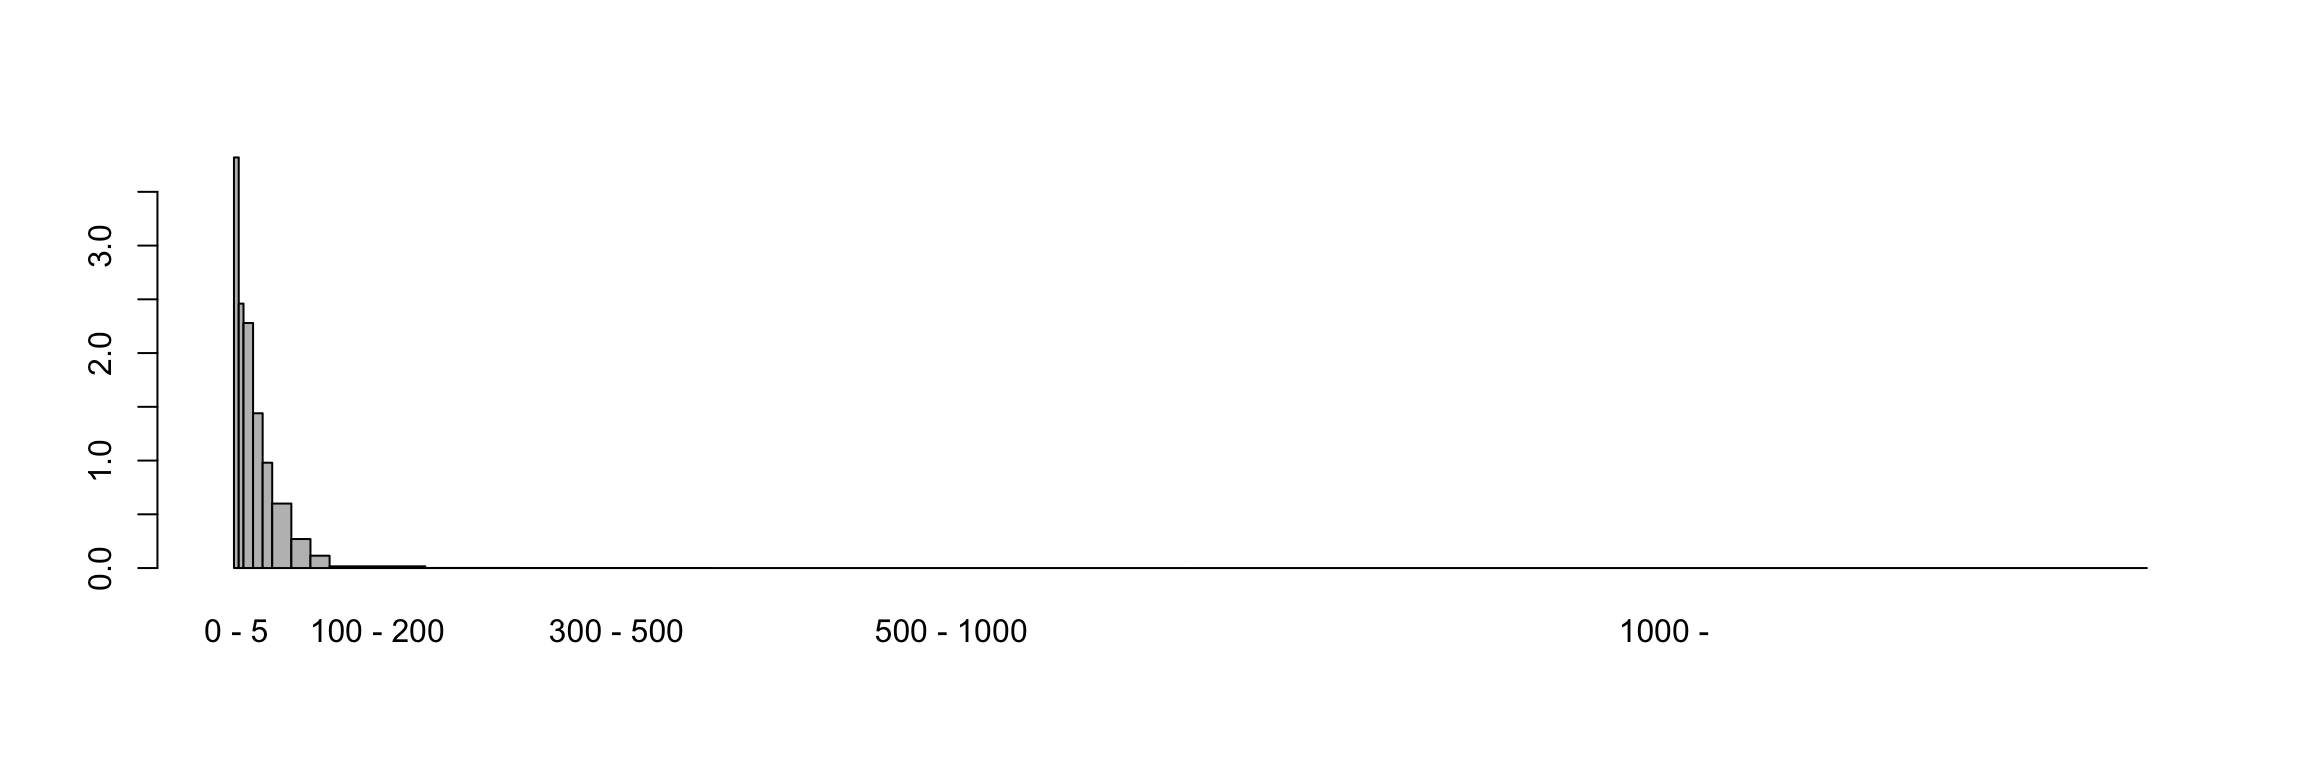
\includegraphics{Gini_OECD_files/figure-latex/unnamed-chunk-6-1.pdf}

\begin{itemize}
\tightlist
\item
  개선도 순서(내림차순)를 \texttt{o\_improvement}로 저장하여 지속적으로
  활용.
\end{itemize}

\begin{Shaded}
\begin{Highlighting}[]
\NormalTok{o\_improvement }\OtherTok{\textless{}{-}} \FunctionTok{order}\NormalTok{(Gini\_b\_a}\SpecialCharTok{$}\NormalTok{Improvement, }\AttributeTok{decreasing =} \ConstantTok{TRUE}\NormalTok{)}
\NormalTok{Gini\_b\_a}\SpecialCharTok{$}\NormalTok{Country[o\_improvement]}
\end{Highlighting}
\end{Shaded}

\begin{verbatim}
##  [1] "Austria"         "Belgium"         "Germany"         "Finland"        
##  [5] "Italy"           "Hungary"         "Luxembourg"      "France"         
##  [9] "Czech_Republic"  "Slovenia"        "Portugal"        "Denmark"        
## [13] "Sweden"          "Poland"          "Norway"          "Slovak_Republic"
## [17] "Spain"           "Estonia"         "Japan"           "Australia"      
## [21] "Netherlands"     "Greece"          "Israel"          "New_Zealand"    
## [25] "Canada"          "United_Kingdom"  "United_States"   "Switzerland"    
## [29] "Iceland"         "Turkey"          "Chile"           "South_Korea"    
## [33] "Mexico"          "Ireland"
\end{verbatim}

\begin{itemize}
\tightlist
\item
  개선도 순서대로 막대를 늘어세우면,
\end{itemize}

\begin{Shaded}
\begin{Highlighting}[]
\FunctionTok{barplot}\NormalTok{(}\FunctionTok{as.matrix}\NormalTok{(}\FunctionTok{t}\NormalTok{(Gini\_b\_a[o\_improvement, }\DecValTok{2}\SpecialCharTok{:}\DecValTok{3}\NormalTok{])), }
        \AttributeTok{beside =} \ConstantTok{TRUE}\NormalTok{, }
        \AttributeTok{names.arg =}\NormalTok{ Gini\_b\_a}\SpecialCharTok{$}\NormalTok{Country[o\_improvement])}
\end{Highlighting}
\end{Shaded}

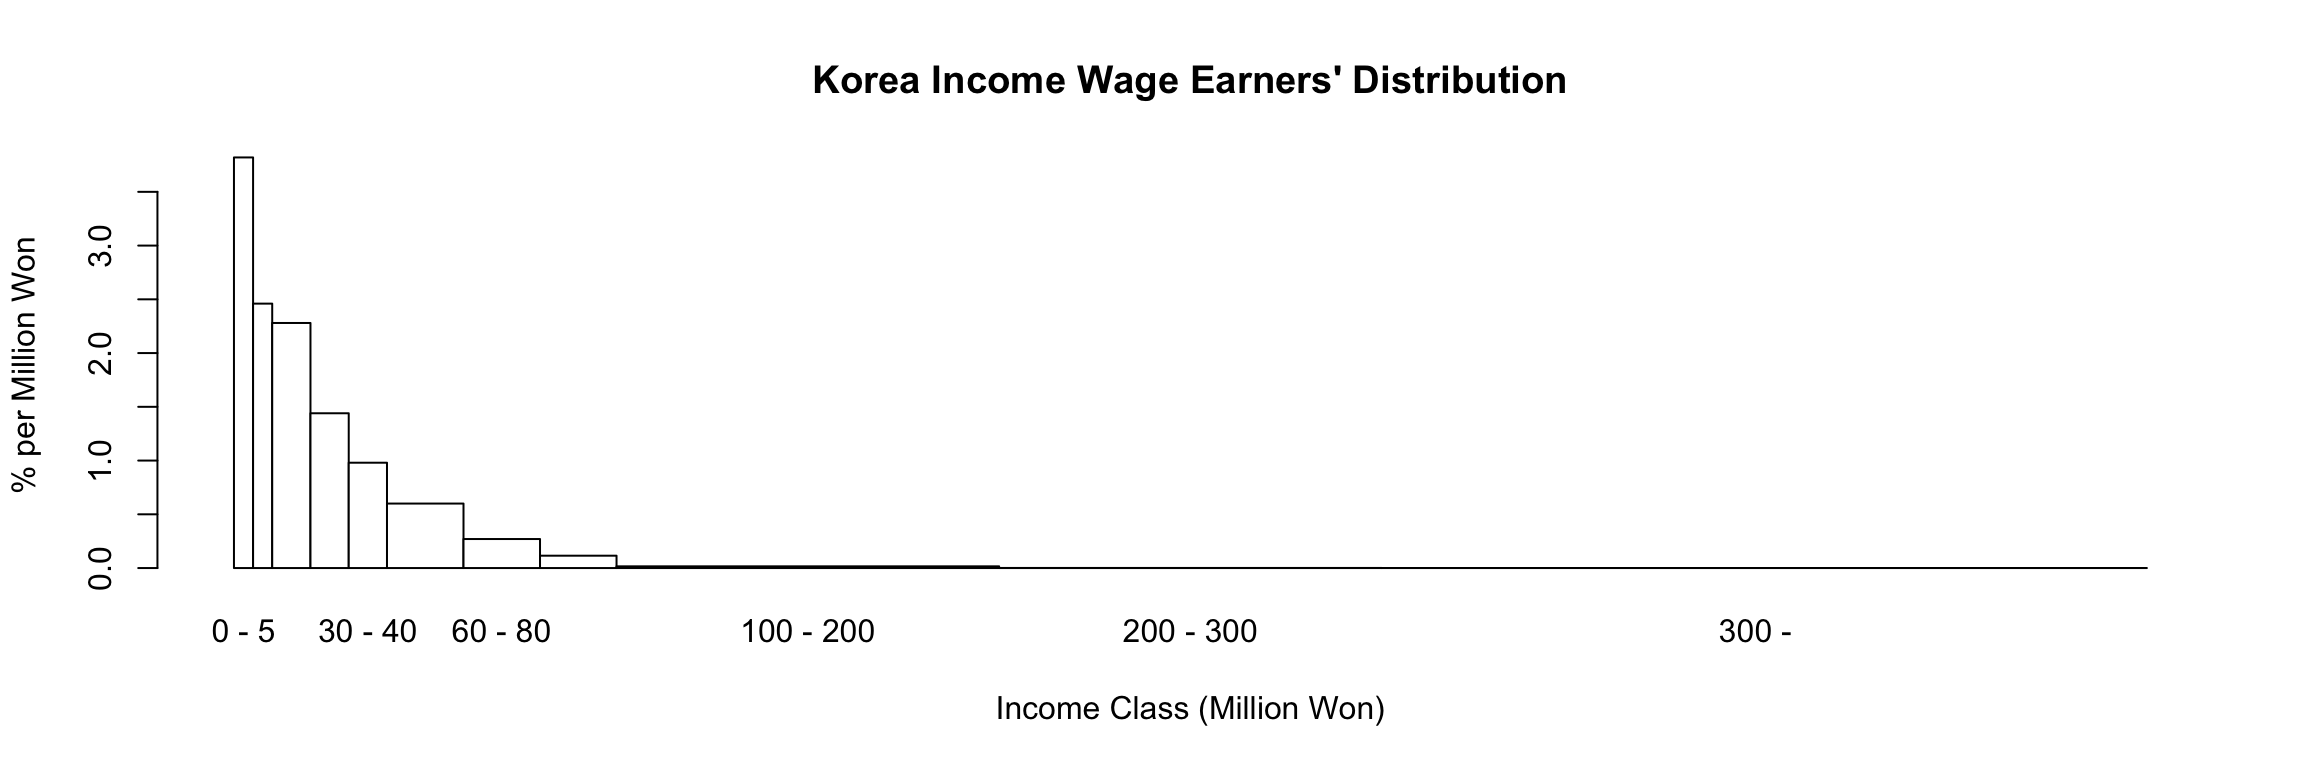
\includegraphics{Gini_OECD_files/figure-latex/unnamed-chunk-8-1.pdf}

\begin{itemize}
\tightlist
\item
  \texttt{las\ =\ 2}를 이용하여 막대 이름을 눕힘.
\end{itemize}

\begin{Shaded}
\begin{Highlighting}[]
\FunctionTok{barplot}\NormalTok{(}\FunctionTok{as.matrix}\NormalTok{(}\FunctionTok{t}\NormalTok{(Gini\_b\_a[o\_improvement, }\DecValTok{2}\SpecialCharTok{:}\DecValTok{3}\NormalTok{])), }
        \AttributeTok{beside =} \ConstantTok{TRUE}\NormalTok{, }
        \AttributeTok{names.arg =}\NormalTok{ Gini\_b\_a}\SpecialCharTok{$}\NormalTok{Country[o\_improvement], }
        \AttributeTok{las =} \DecValTok{2}\NormalTok{)}
\end{Highlighting}
\end{Shaded}

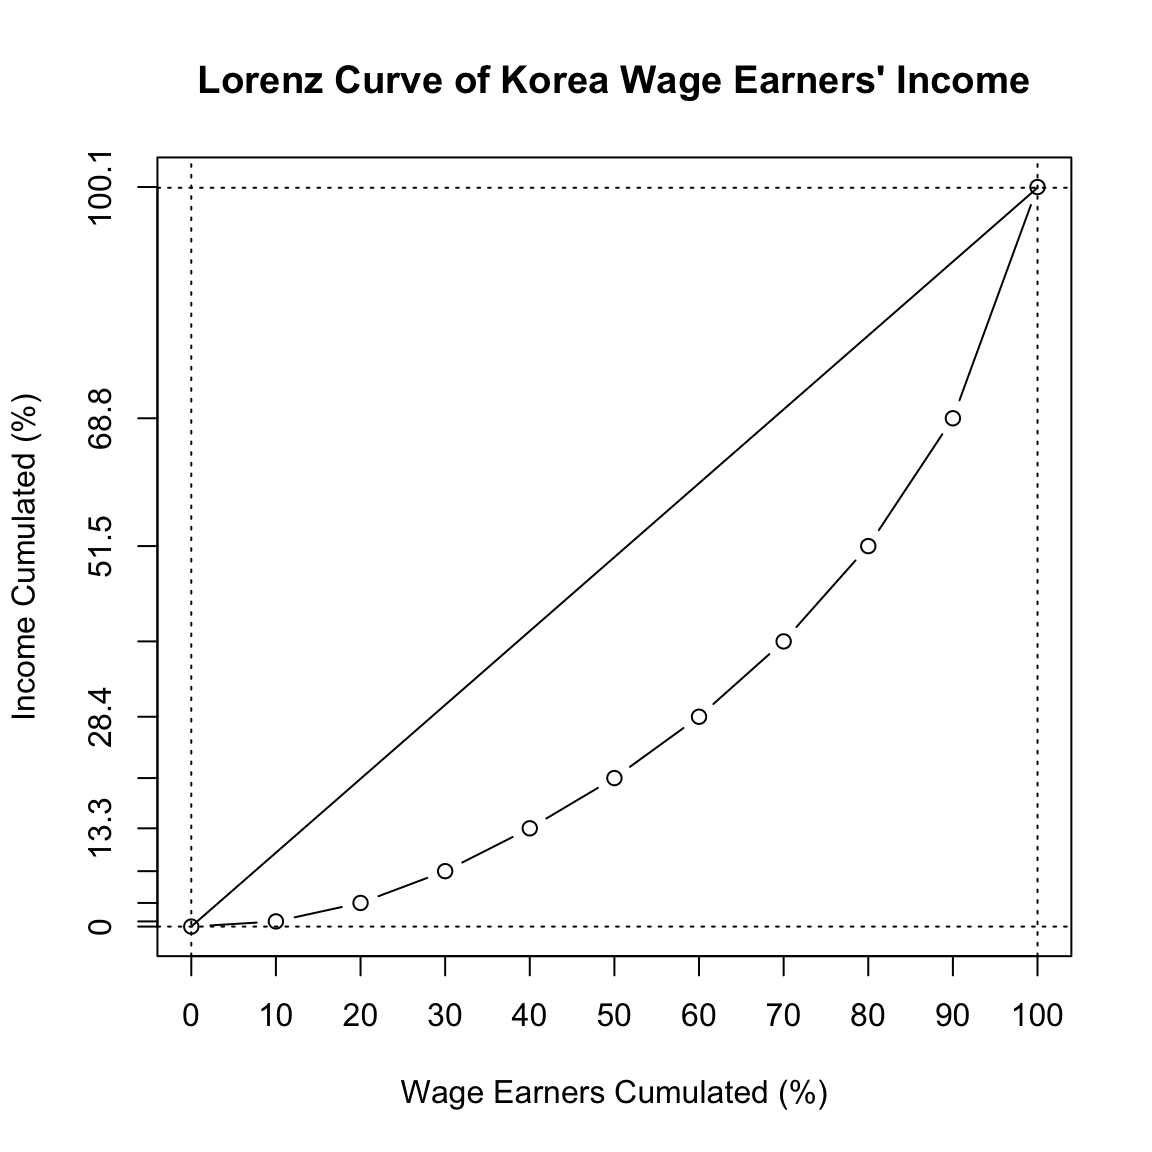
\includegraphics{Gini_OECD_files/figure-latex/unnamed-chunk-9-1.pdf}

\begin{itemize}
\tightlist
\item
  나라 이름이 가리지 않도록 \texttt{par("mai")}를 조정
\end{itemize}

\begin{Shaded}
\begin{Highlighting}[]
\NormalTok{old\_par }\OtherTok{\textless{}{-}} \FunctionTok{par}\NormalTok{(}\AttributeTok{no.readonly =} \ConstantTok{TRUE}\NormalTok{)}
\FunctionTok{par}\NormalTok{(}\StringTok{"mai"}\NormalTok{)}
\end{Highlighting}
\end{Shaded}

\begin{verbatim}
## [1] 1.02 0.82 0.82 0.42
\end{verbatim}

\begin{Shaded}
\begin{Highlighting}[]
\FunctionTok{par}\NormalTok{(}\StringTok{"mai"} \OtherTok{=} \FunctionTok{c}\NormalTok{(}\FloatTok{1.5}\NormalTok{, }\FloatTok{0.8}\NormalTok{, }\FloatTok{0.8}\NormalTok{, }\FloatTok{0.4}\NormalTok{))}
\FunctionTok{barplot}\NormalTok{(}\FunctionTok{as.matrix}\NormalTok{(}\FunctionTok{t}\NormalTok{(Gini\_b\_a[o\_improvement, }\DecValTok{2}\SpecialCharTok{:}\DecValTok{3}\NormalTok{])), }
        \AttributeTok{beside =} \ConstantTok{TRUE}\NormalTok{, }
        \AttributeTok{names.arg =}\NormalTok{ Gini\_b\_a}\SpecialCharTok{$}\NormalTok{Country[o\_improvement], }
        \AttributeTok{las =} \DecValTok{2}\NormalTok{)}
\end{Highlighting}
\end{Shaded}

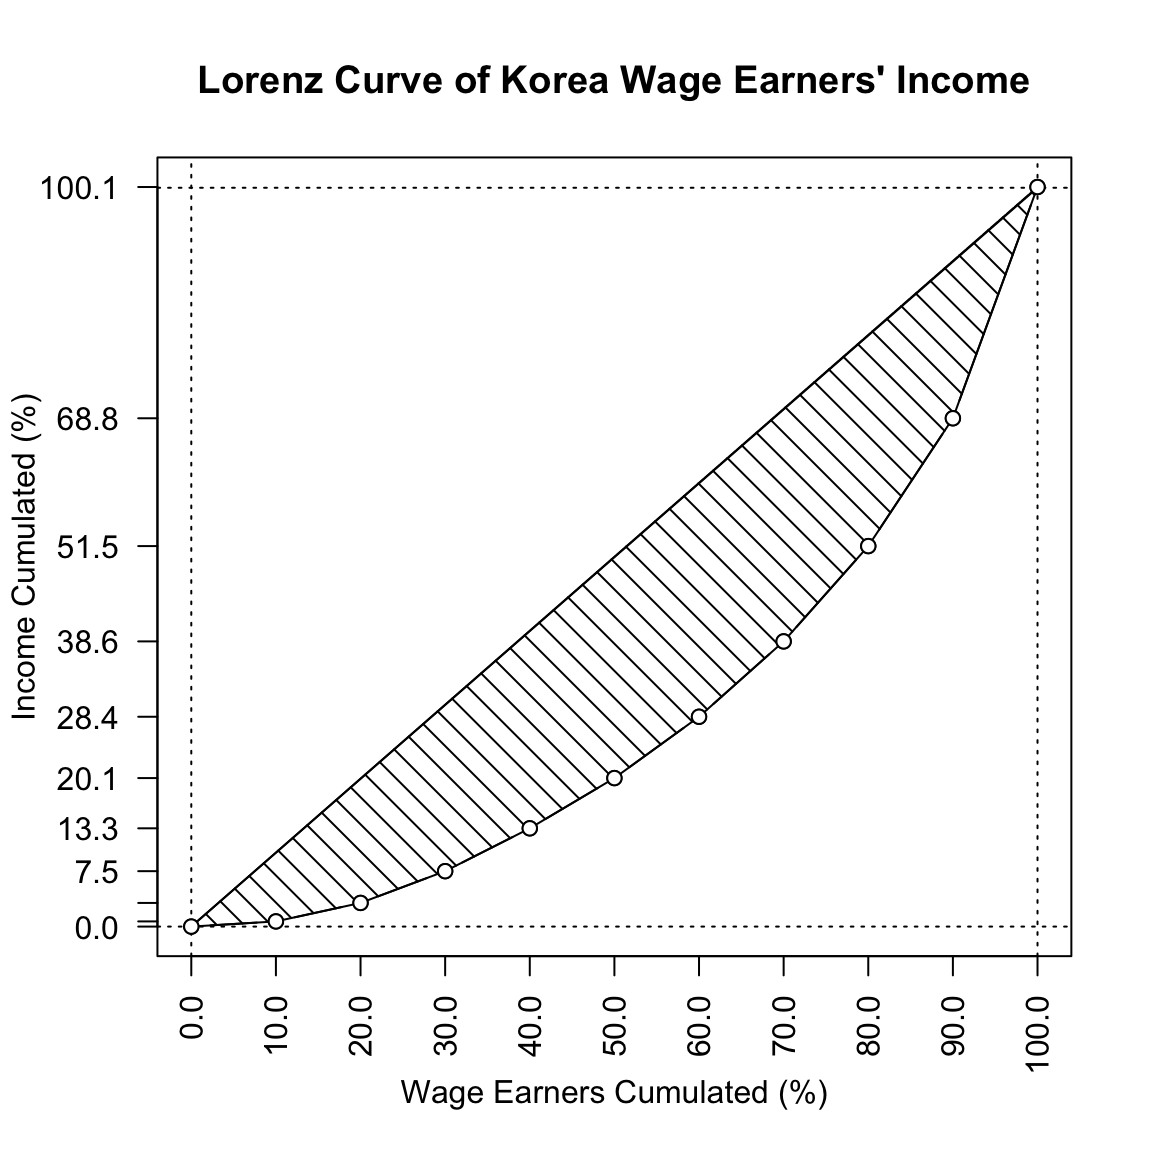
\includegraphics{Gini_OECD_files/figure-latex/unnamed-chunk-10-1.pdf}

\begin{Shaded}
\begin{Highlighting}[]
\FunctionTok{par}\NormalTok{(old\_par)}
\end{Highlighting}
\end{Shaded}

\begin{itemize}
\tightlist
\item
  불평등이 심하다고 판단하는 Gini 계수 0.4를 경계로 나눠 보면,
\end{itemize}

\begin{Shaded}
\begin{Highlighting}[]
\NormalTok{old\_par }\OtherTok{\textless{}{-}} \FunctionTok{par}\NormalTok{(}\AttributeTok{no.readonly =} \ConstantTok{TRUE}\NormalTok{)}
\FunctionTok{par}\NormalTok{(}\StringTok{"mai"}\NormalTok{)}
\end{Highlighting}
\end{Shaded}

\begin{verbatim}
## [1] 1.02 0.82 0.82 0.42
\end{verbatim}

\begin{Shaded}
\begin{Highlighting}[]
\FunctionTok{par}\NormalTok{(}\StringTok{"mai"} \OtherTok{=} \FunctionTok{c}\NormalTok{(}\FloatTok{1.5}\NormalTok{, }\FloatTok{0.8}\NormalTok{, }\FloatTok{0.8}\NormalTok{, }\FloatTok{0.4}\NormalTok{))}
\FunctionTok{barplot}\NormalTok{(}\FunctionTok{as.matrix}\NormalTok{(}\FunctionTok{t}\NormalTok{(Gini\_b\_a[o\_improvement, }\DecValTok{2}\SpecialCharTok{:}\DecValTok{3}\NormalTok{])), }
        \AttributeTok{beside =} \ConstantTok{TRUE}\NormalTok{, }
        \AttributeTok{names.arg =}\NormalTok{ Gini\_b\_a}\SpecialCharTok{$}\NormalTok{Country[o\_improvement], }
        \AttributeTok{las =} \DecValTok{2}\NormalTok{)}
\FunctionTok{abline}\NormalTok{(}\AttributeTok{h =} \FloatTok{0.4}\NormalTok{, }\AttributeTok{lty =} \DecValTok{2}\NormalTok{, }\AttributeTok{col =} \StringTok{"red"}\NormalTok{)}
\end{Highlighting}
\end{Shaded}

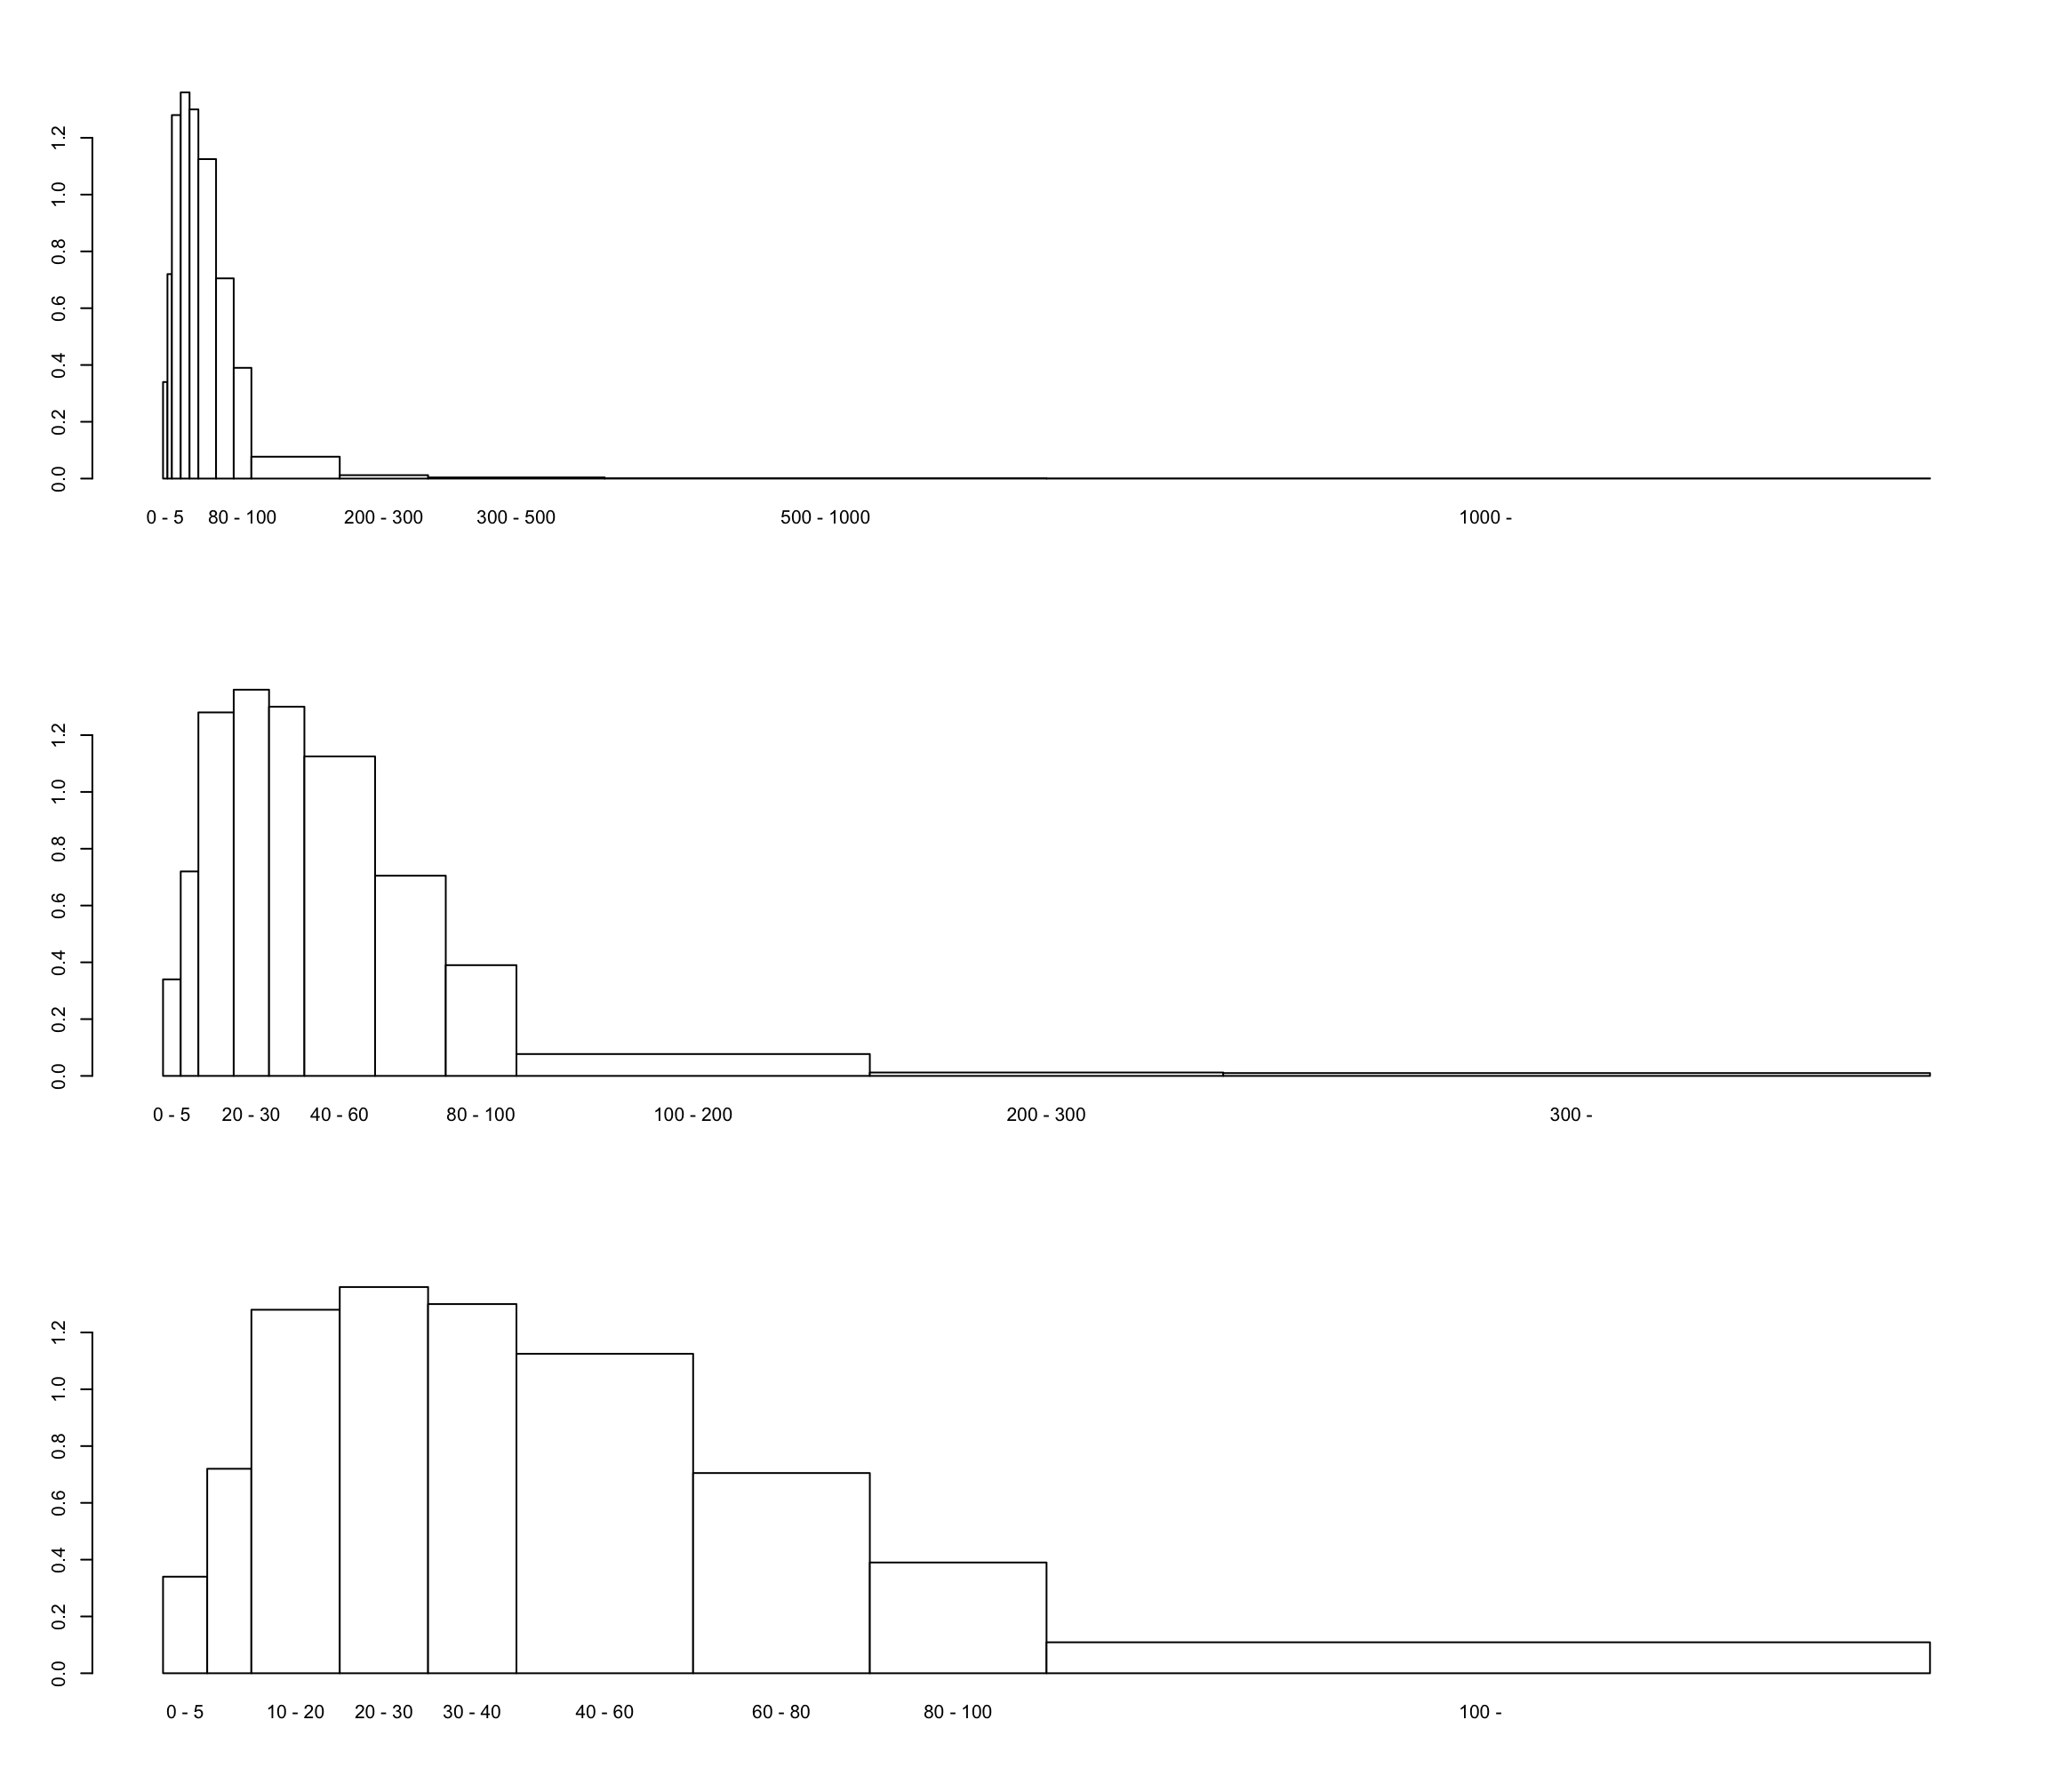
\includegraphics{Gini_OECD_files/figure-latex/unnamed-chunk-11-1.pdf}

\begin{Shaded}
\begin{Highlighting}[]
\FunctionTok{par}\NormalTok{(old\_par)}
\end{Highlighting}
\end{Shaded}

\begin{itemize}
\tightlist
\item
  범례와 메인 타이틀 추가. 좌표에 유의
\end{itemize}

\begin{Shaded}
\begin{Highlighting}[]
\NormalTok{old\_par }\OtherTok{\textless{}{-}} \FunctionTok{par}\NormalTok{(}\AttributeTok{no.readonly =} \ConstantTok{TRUE}\NormalTok{)}
\FunctionTok{par}\NormalTok{(}\StringTok{"mai"}\NormalTok{)}
\end{Highlighting}
\end{Shaded}

\begin{verbatim}
## [1] 1.02 0.82 0.82 0.42
\end{verbatim}

\begin{Shaded}
\begin{Highlighting}[]
\FunctionTok{par}\NormalTok{(}\StringTok{"mai"} \OtherTok{=} \FunctionTok{c}\NormalTok{(}\FloatTok{1.5}\NormalTok{, }\FloatTok{0.8}\NormalTok{, }\FloatTok{0.8}\NormalTok{, }\FloatTok{0.4}\NormalTok{))}
\FunctionTok{barplot}\NormalTok{(}\FunctionTok{as.matrix}\NormalTok{(}\FunctionTok{t}\NormalTok{(Gini\_b\_a[o\_improvement, }\DecValTok{2}\SpecialCharTok{:}\DecValTok{3}\NormalTok{])), }
        \AttributeTok{beside =} \ConstantTok{TRUE}\NormalTok{, }
        \AttributeTok{names.arg =}\NormalTok{ Gini\_b\_a}\SpecialCharTok{$}\NormalTok{Country[o\_improvement], }
        \AttributeTok{legend.text =} \FunctionTok{c}\NormalTok{(}\StringTok{"Before Tax"}\NormalTok{, }\StringTok{"After Tax"}\NormalTok{),}
        \AttributeTok{args.legend =} \FunctionTok{list}\NormalTok{(}\AttributeTok{x =} \DecValTok{105}\NormalTok{, }\AttributeTok{y =} \FloatTok{0.62}\NormalTok{), }
        \AttributeTok{las =} \DecValTok{2}\NormalTok{)}
\FunctionTok{abline}\NormalTok{(}\AttributeTok{h =} \FloatTok{0.4}\NormalTok{, }\AttributeTok{lty =} \DecValTok{2}\NormalTok{, }\AttributeTok{col =} \StringTok{"red"}\NormalTok{)}
\FunctionTok{title}\NormalTok{(}\AttributeTok{main =} \StringTok{"Gini Coefficients of OECD Countries"}\NormalTok{)}
\end{Highlighting}
\end{Shaded}

\includegraphics{Gini_OECD_files/figure-latex/unnamed-chunk-12-1.pdf}

\begin{Shaded}
\begin{Highlighting}[]
\FunctionTok{par}\NormalTok{(old\_par)}
\end{Highlighting}
\end{Shaded}

\begin{itemize}
\tightlist
\item
  이번에는 막대를 눕히는 방법을 생각해 보자. 옆으로 눕히면서
  \texttt{las\ =\ 1} 로 설정하면,
\end{itemize}

\begin{Shaded}
\begin{Highlighting}[]
\FunctionTok{barplot}\NormalTok{(}\FunctionTok{as.matrix}\NormalTok{(}\FunctionTok{t}\NormalTok{(Gini\_b\_a[o\_improvement, }\DecValTok{2}\SpecialCharTok{:}\DecValTok{3}\NormalTok{])), }
        \AttributeTok{beside =} \ConstantTok{TRUE}\NormalTok{, }
        \AttributeTok{horiz =} \ConstantTok{TRUE}\NormalTok{, }
        \AttributeTok{names.arg =}\NormalTok{ Gini\_b\_a}\SpecialCharTok{$}\NormalTok{Country[o\_improvement], }
        \AttributeTok{las =} \DecValTok{1}\NormalTok{)}
\end{Highlighting}
\end{Shaded}

\includegraphics{Gini_OECD_files/figure-latex/unnamed-chunk-13-1.pdf}

\begin{itemize}
\tightlist
\item
  역시 나라 이름이 가리지 않도록 \texttt{par("mai")}를 조정.
\end{itemize}

\begin{Shaded}
\begin{Highlighting}[]
\NormalTok{old\_par }\OtherTok{\textless{}{-}} \FunctionTok{par}\NormalTok{(}\AttributeTok{no.readonly =} \ConstantTok{TRUE}\NormalTok{)}
\FunctionTok{par}\NormalTok{(}\StringTok{"mai"}\NormalTok{)}
\end{Highlighting}
\end{Shaded}

\begin{verbatim}
## [1] 1.02 0.82 0.82 0.42
\end{verbatim}

\begin{Shaded}
\begin{Highlighting}[]
\FunctionTok{par}\NormalTok{(}\StringTok{"mai"} \OtherTok{=} \FunctionTok{c}\NormalTok{(}\FloatTok{1.0}\NormalTok{, }\FloatTok{1.5}\NormalTok{, }\FloatTok{0.8}\NormalTok{, }\FloatTok{0.4}\NormalTok{))}
\FunctionTok{barplot}\NormalTok{(}\FunctionTok{as.matrix}\NormalTok{(}\FunctionTok{t}\NormalTok{(Gini\_b\_a[o\_improvement, }\DecValTok{2}\SpecialCharTok{:}\DecValTok{3}\NormalTok{])), }
        \AttributeTok{beside =} \ConstantTok{TRUE}\NormalTok{, }
        \AttributeTok{horiz =} \ConstantTok{TRUE}\NormalTok{, }
        \AttributeTok{names.arg =}\NormalTok{ Gini\_b\_a}\SpecialCharTok{$}\NormalTok{Country[o\_improvement], }
        \AttributeTok{las =} \DecValTok{1}\NormalTok{)}
\end{Highlighting}
\end{Shaded}

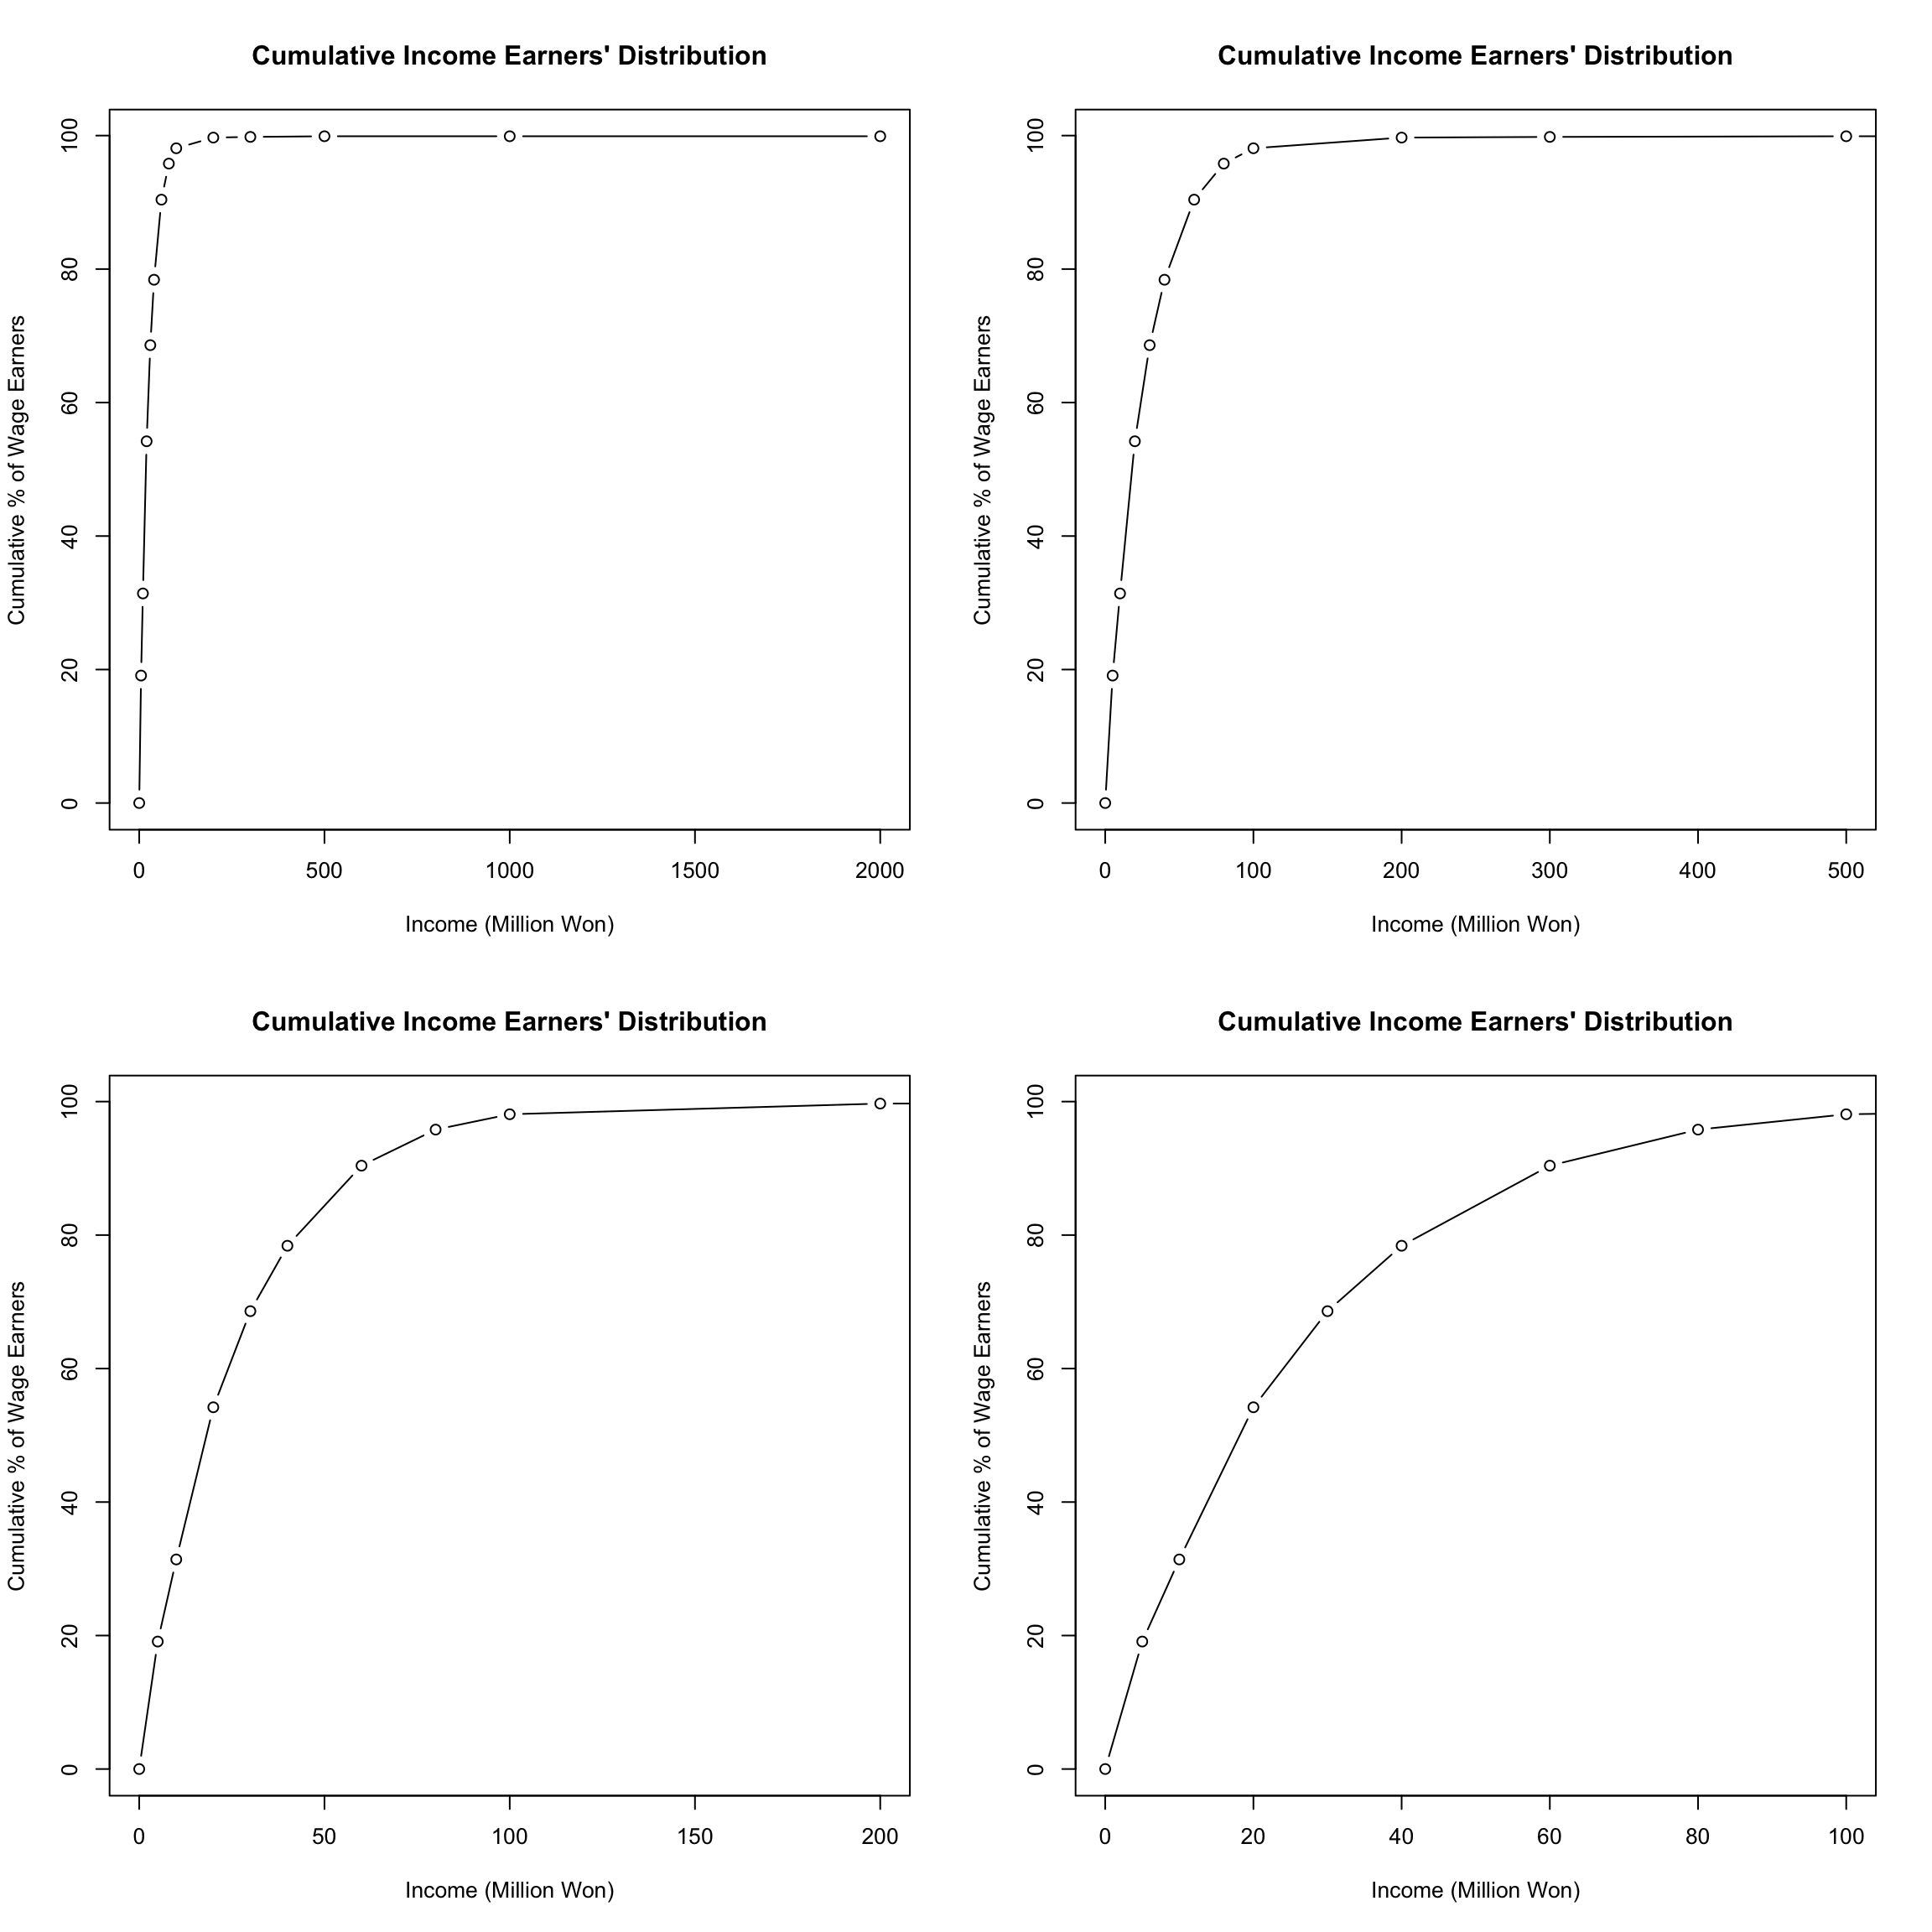
\includegraphics{Gini_OECD_files/figure-latex/unnamed-chunk-14-1.pdf}

\begin{Shaded}
\begin{Highlighting}[]
\FunctionTok{par}\NormalTok{(old\_par)}
\end{Highlighting}
\end{Shaded}

\begin{itemize}
\tightlist
\item
  개선도가 낮은 순서대로 밑에서 올라가도록 다시 그리면,
\end{itemize}

\begin{Shaded}
\begin{Highlighting}[]
\NormalTok{old\_par }\OtherTok{\textless{}{-}} \FunctionTok{par}\NormalTok{(}\AttributeTok{no.readonly =} \ConstantTok{TRUE}\NormalTok{)}
\FunctionTok{par}\NormalTok{(}\StringTok{"mai"}\NormalTok{)}
\end{Highlighting}
\end{Shaded}

\begin{verbatim}
## [1] 1.02 0.82 0.82 0.42
\end{verbatim}

\begin{Shaded}
\begin{Highlighting}[]
\FunctionTok{par}\NormalTok{(}\StringTok{"mai"} \OtherTok{=} \FunctionTok{c}\NormalTok{(}\FloatTok{1.0}\NormalTok{, }\FloatTok{1.5}\NormalTok{, }\FloatTok{0.8}\NormalTok{, }\FloatTok{0.4}\NormalTok{))}
\FunctionTok{barplot}\NormalTok{(}\FunctionTok{as.matrix}\NormalTok{(}\FunctionTok{t}\NormalTok{(Gini\_b\_a[}\FunctionTok{order}\NormalTok{(Gini\_b\_a}\SpecialCharTok{$}\NormalTok{Improvement, }
                                   \AttributeTok{na.last =} \ConstantTok{FALSE}\NormalTok{), }\DecValTok{2}\SpecialCharTok{:}\DecValTok{3}\NormalTok{])), }
        \AttributeTok{beside =} \ConstantTok{TRUE}\NormalTok{, }
        \AttributeTok{horiz =} \ConstantTok{TRUE}\NormalTok{, }
        \AttributeTok{names.arg =}\NormalTok{ Gini\_b\_a}\SpecialCharTok{$}\NormalTok{Country[}\FunctionTok{order}\NormalTok{(Gini\_b\_a}\SpecialCharTok{$}\NormalTok{Improvement, }
                                           \AttributeTok{na.last =} \ConstantTok{FALSE}\NormalTok{)], }
        \AttributeTok{las =} \DecValTok{1}\NormalTok{)}
\end{Highlighting}
\end{Shaded}

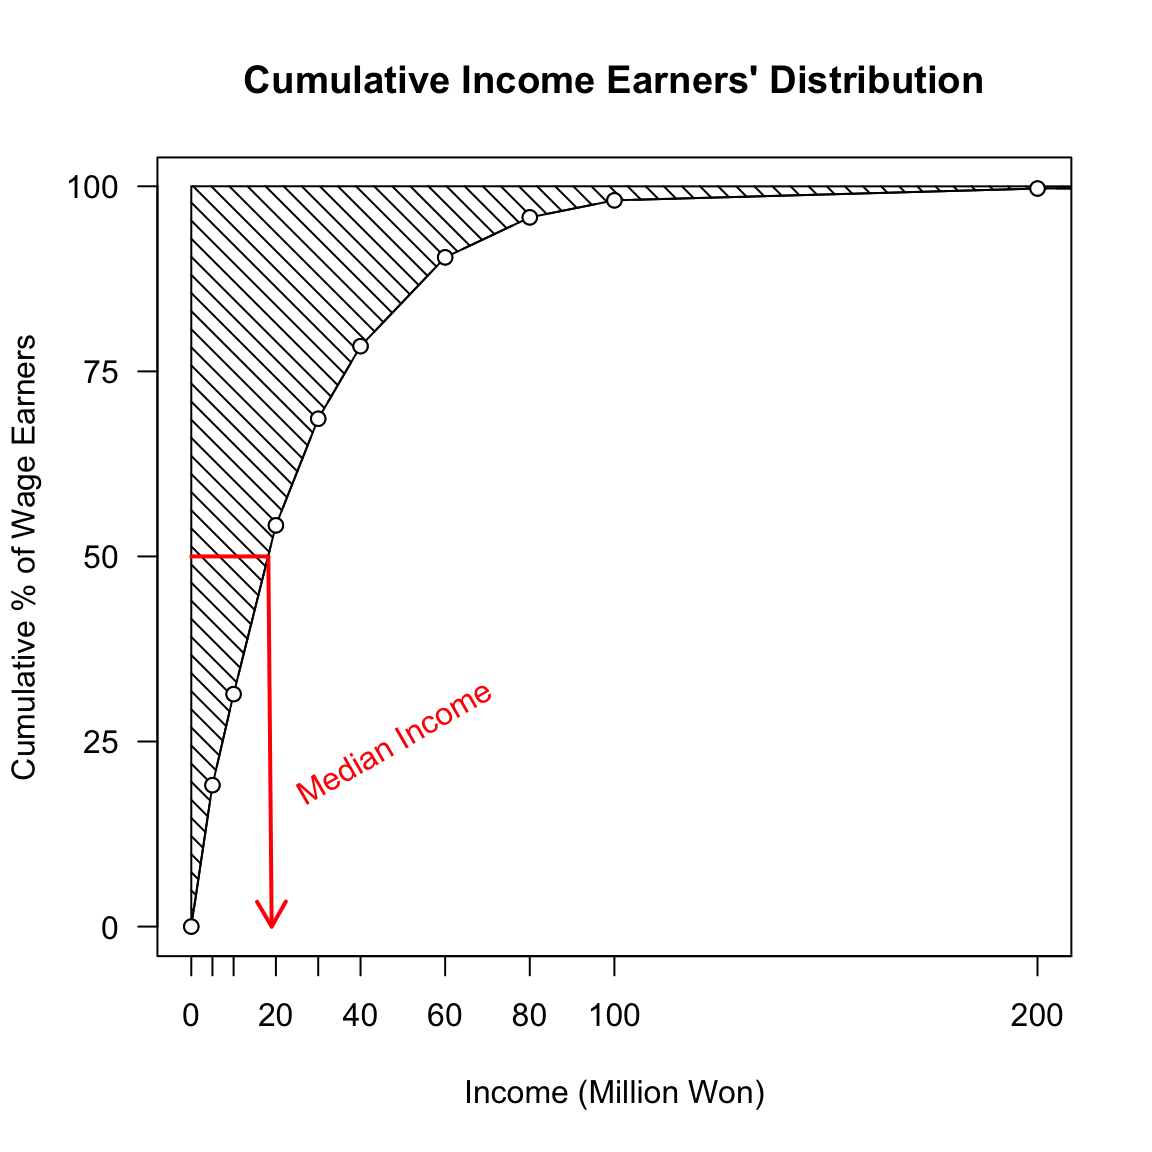
\includegraphics{Gini_OECD_files/figure-latex/unnamed-chunk-15-1.pdf}

\begin{Shaded}
\begin{Highlighting}[]
\FunctionTok{par}\NormalTok{(old\_par)}
\end{Highlighting}
\end{Shaded}

\begin{itemize}
\tightlist
\item
  이 때, Ireland가 맨 위에 올라오는 게 보기 좋지 않으므로,
  \texttt{na.last\ =\ FALSE}를 추가한 것임.

  \begin{itemize}
  \tightlist
  \item
    세전 Gini 계수 0.4를 경계로 나눠보면
  \end{itemize}
\end{itemize}

\begin{Shaded}
\begin{Highlighting}[]
\NormalTok{old\_par }\OtherTok{\textless{}{-}} \FunctionTok{par}\NormalTok{(}\AttributeTok{no.readonly =} \ConstantTok{TRUE}\NormalTok{)}
\FunctionTok{par}\NormalTok{(}\StringTok{"mai"}\NormalTok{)}
\end{Highlighting}
\end{Shaded}

\begin{verbatim}
## [1] 1.02 0.82 0.82 0.42
\end{verbatim}

\begin{Shaded}
\begin{Highlighting}[]
\FunctionTok{par}\NormalTok{(}\StringTok{"mai"} \OtherTok{=} \FunctionTok{c}\NormalTok{(}\FloatTok{1.0}\NormalTok{, }\FloatTok{1.5}\NormalTok{, }\FloatTok{0.8}\NormalTok{, }\FloatTok{0.4}\NormalTok{))}
\FunctionTok{barplot}\NormalTok{(}\FunctionTok{as.matrix}\NormalTok{(}\FunctionTok{t}\NormalTok{(Gini\_b\_a[}\FunctionTok{order}\NormalTok{(Gini\_b\_a}\SpecialCharTok{$}\NormalTok{Improvement, }
                                   \AttributeTok{na.last =} \ConstantTok{FALSE}\NormalTok{), }\DecValTok{2}\SpecialCharTok{:}\DecValTok{3}\NormalTok{])), }
        \AttributeTok{beside =} \ConstantTok{TRUE}\NormalTok{, }
        \AttributeTok{horiz =} \ConstantTok{TRUE}\NormalTok{, }
        \AttributeTok{names.arg =}\NormalTok{ Gini\_b\_a}\SpecialCharTok{$}\NormalTok{Country[}\FunctionTok{order}\NormalTok{(Gini\_b\_a}\SpecialCharTok{$}\NormalTok{Improvement, }
                                           \AttributeTok{na.last =} \ConstantTok{FALSE}\NormalTok{)],}
        \AttributeTok{las =} \DecValTok{1}\NormalTok{)}
\FunctionTok{abline}\NormalTok{(}\AttributeTok{v =} \FloatTok{0.4}\NormalTok{, }\AttributeTok{lty =} \DecValTok{2}\NormalTok{, }\AttributeTok{col =} \StringTok{"red"}\NormalTok{)}
\end{Highlighting}
\end{Shaded}

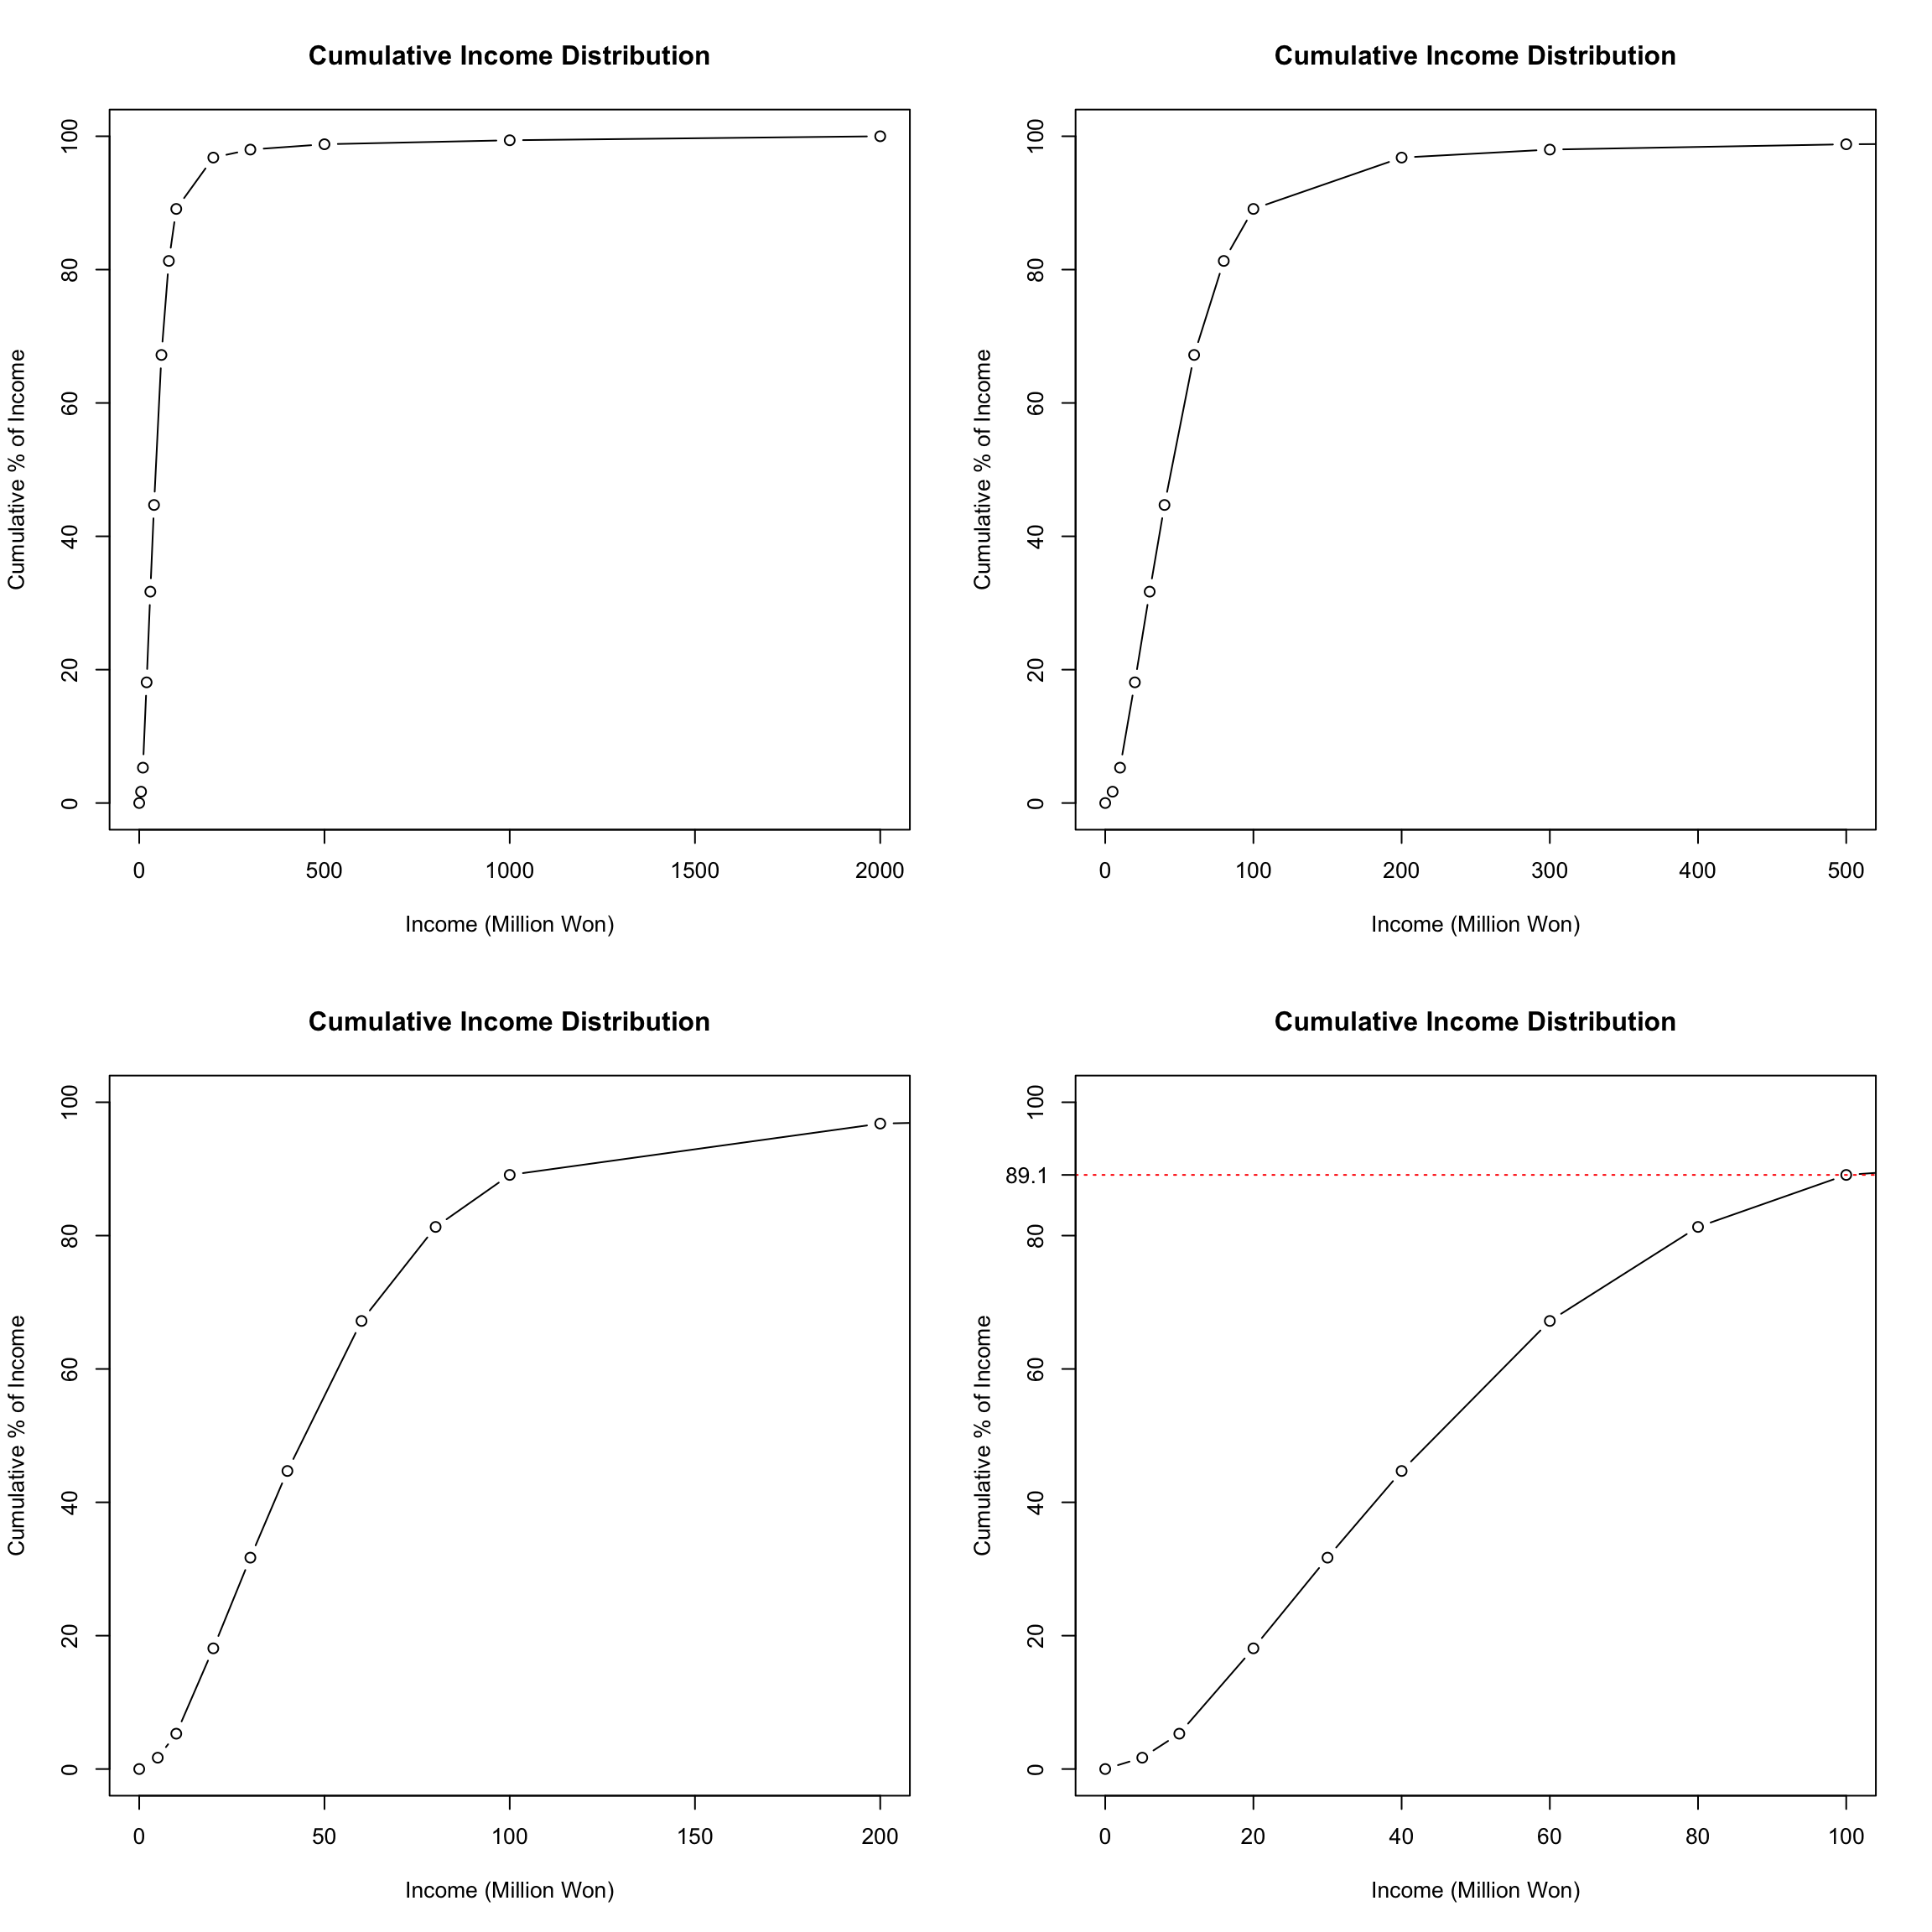
\includegraphics{Gini_OECD_files/figure-latex/unnamed-chunk-16-1.pdf}

\begin{Shaded}
\begin{Highlighting}[]
\FunctionTok{par}\NormalTok{(old\_par)}
\end{Highlighting}
\end{Shaded}

\begin{itemize}
\tightlist
\item
  범례 및 메인 타이틀 추가. 시행착오를 거쳐 구한 좌표에 유의할 것.
\end{itemize}

\begin{Shaded}
\begin{Highlighting}[]
\NormalTok{old\_par }\OtherTok{\textless{}{-}} \FunctionTok{par}\NormalTok{(}\AttributeTok{no.readonly =} \ConstantTok{TRUE}\NormalTok{)}
\FunctionTok{par}\NormalTok{(}\StringTok{"mai"}\NormalTok{)}
\end{Highlighting}
\end{Shaded}

\begin{verbatim}
## [1] 1.02 0.82 0.82 0.42
\end{verbatim}

\begin{Shaded}
\begin{Highlighting}[]
\FunctionTok{par}\NormalTok{(}\StringTok{"mai"} \OtherTok{=} \FunctionTok{c}\NormalTok{(}\FloatTok{1.0}\NormalTok{, }\FloatTok{1.5}\NormalTok{, }\FloatTok{0.8}\NormalTok{, }\FloatTok{0.8}\NormalTok{))}
\FunctionTok{barplot}\NormalTok{(}\FunctionTok{as.matrix}\NormalTok{(}\FunctionTok{t}\NormalTok{(Gini\_b\_a[}\FunctionTok{order}\NormalTok{(Gini\_b\_a}\SpecialCharTok{$}\NormalTok{Improvement, }
                                   \AttributeTok{na.last =} \ConstantTok{FALSE}\NormalTok{), }\DecValTok{2}\SpecialCharTok{:}\DecValTok{3}\NormalTok{])), }
        \AttributeTok{beside =} \ConstantTok{TRUE}\NormalTok{, }
        \AttributeTok{horiz =} \ConstantTok{TRUE}\NormalTok{, }
        \AttributeTok{names.arg =}\NormalTok{ Gini\_b\_a}\SpecialCharTok{$}\NormalTok{Country[}\FunctionTok{order}\NormalTok{(Gini\_b\_a}\SpecialCharTok{$}\NormalTok{Improvement, }
                                           \AttributeTok{na.last =} \ConstantTok{FALSE}\NormalTok{)],}
        \AttributeTok{legend.text =} \FunctionTok{c}\NormalTok{(}\StringTok{"Before Tax"}\NormalTok{, }\StringTok{"After Tax"}\NormalTok{), }
        \AttributeTok{args.legend =} \FunctionTok{list}\NormalTok{(}\AttributeTok{x =} \FloatTok{0.67}\NormalTok{, }\AttributeTok{y =} \DecValTok{110}\NormalTok{), }
        \AttributeTok{las =} \DecValTok{1}\NormalTok{)}
\FunctionTok{abline}\NormalTok{(}\AttributeTok{v =} \FloatTok{0.4}\NormalTok{, }\AttributeTok{lty =} \DecValTok{2}\NormalTok{, }\AttributeTok{col =} \StringTok{"red"}\NormalTok{)}
\FunctionTok{title}\NormalTok{(}\AttributeTok{main =} \StringTok{"Gini Coefficients of OECD Countries"}\NormalTok{)}
\end{Highlighting}
\end{Shaded}

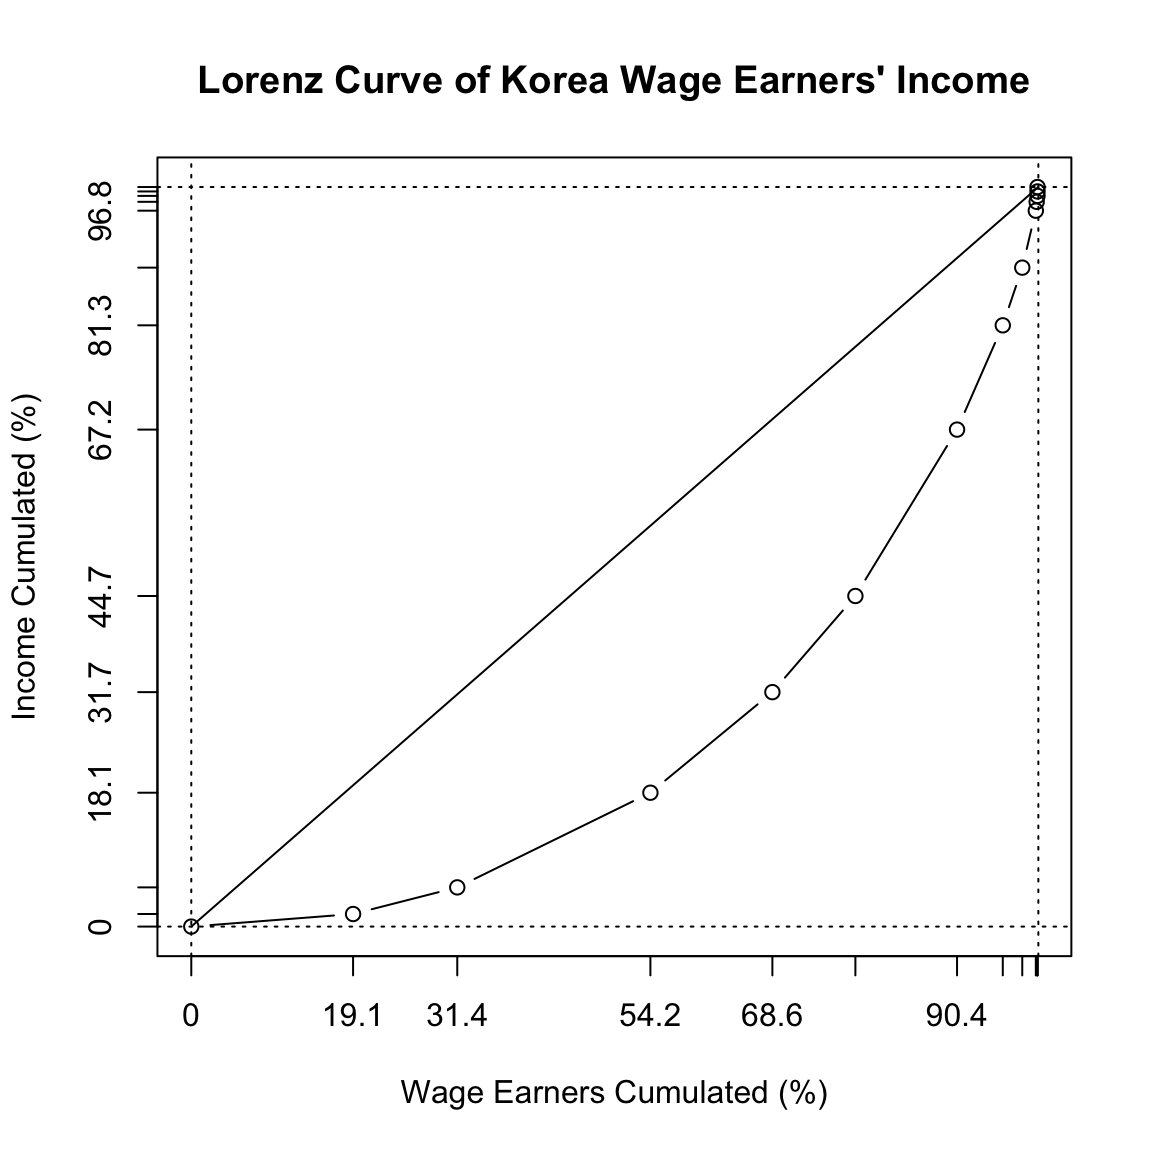
\includegraphics{Gini_OECD_files/figure-latex/unnamed-chunk-17-1.pdf}

\begin{Shaded}
\begin{Highlighting}[]
\FunctionTok{par}\NormalTok{(old\_par)}
\end{Highlighting}
\end{Shaded}

\hypertarget{ggplot}{%
\subsection{ggplot}\label{ggplot}}

\hypertarget{data-reshaping}{%
\subsubsection{Data reshaping}\label{data-reshaping}}

\begin{itemize}
\tightlist
\item
  \texttt{reshape2} package 를 검색 목록에 등록
\end{itemize}

\begin{Shaded}
\begin{Highlighting}[]
\CommentTok{\# library(reshape2)}
\CommentTok{\# (Gini\_b\_a\_melt \textless{}{-} melt(Gini\_b\_a, }
\CommentTok{\#                        id.vars = "Country", }
\CommentTok{\#                        measure.vars = c("Before", "After"), }
\CommentTok{\#                        variable.name = "Tax", }
\CommentTok{\#                        value.name = "Gini\_Coef"))}
\CommentTok{\# str(Gini\_b\_a\_melt)}
\NormalTok{Gini\_Coef }\OtherTok{\textless{}{-}} \FunctionTok{c}\NormalTok{(}\FunctionTok{as.matrix}\NormalTok{(Gini\_b\_a[, }\DecValTok{2}\SpecialCharTok{:}\DecValTok{3}\NormalTok{]))}
\NormalTok{N }\OtherTok{\textless{}{-}} \FunctionTok{length}\NormalTok{(Gini\_Coef)}
\NormalTok{Country }\OtherTok{\textless{}{-}} \FunctionTok{rep}\NormalTok{(Gini\_b\_a[, }\DecValTok{1}\NormalTok{], }\AttributeTok{length.out =}\NormalTok{ N)}
\NormalTok{Tax }\OtherTok{\textless{}{-}} \FunctionTok{gl}\NormalTok{(}\DecValTok{2}\NormalTok{, }\FunctionTok{length}\NormalTok{(Gini\_b\_a[, }\DecValTok{1}\NormalTok{]), N, }
          \AttributeTok{labels =} \FunctionTok{c}\NormalTok{(}\StringTok{"Before"}\NormalTok{, }\StringTok{"After"}\NormalTok{)) }
\NormalTok{Gini\_b\_a\_tbl }\OtherTok{\textless{}{-}} \FunctionTok{data.frame}\NormalTok{(Country, Gini\_Coef, Tax)}
\end{Highlighting}
\end{Shaded}

\begin{itemize}
\tightlist
\item
  \texttt{ggplot2} 등록 후 \texttt{geom\_bar()}
\end{itemize}

\begin{Shaded}
\begin{Highlighting}[]
\FunctionTok{library}\NormalTok{(ggplot2)}
\FunctionTok{ggplot}\NormalTok{(}\AttributeTok{data =}\NormalTok{ Gini\_b\_a\_tbl, }
       \AttributeTok{mapping =} \FunctionTok{aes}\NormalTok{(}\AttributeTok{x =}\NormalTok{ Country, }
                     \AttributeTok{y =}\NormalTok{ Gini\_Coef, }
                     \AttributeTok{fill =}\NormalTok{ Tax)) }\SpecialCharTok{+} 
  \FunctionTok{geom\_bar}\NormalTok{(}\AttributeTok{stat =} \StringTok{"identity"}\NormalTok{, }
           \AttributeTok{position =} \StringTok{"dodge"}\NormalTok{) }\SpecialCharTok{+}
  \FunctionTok{coord\_flip}\NormalTok{()}
\end{Highlighting}
\end{Shaded}

\begin{verbatim}
## Warning: Removed 1 rows containing missing values (geom_bar).
\end{verbatim}

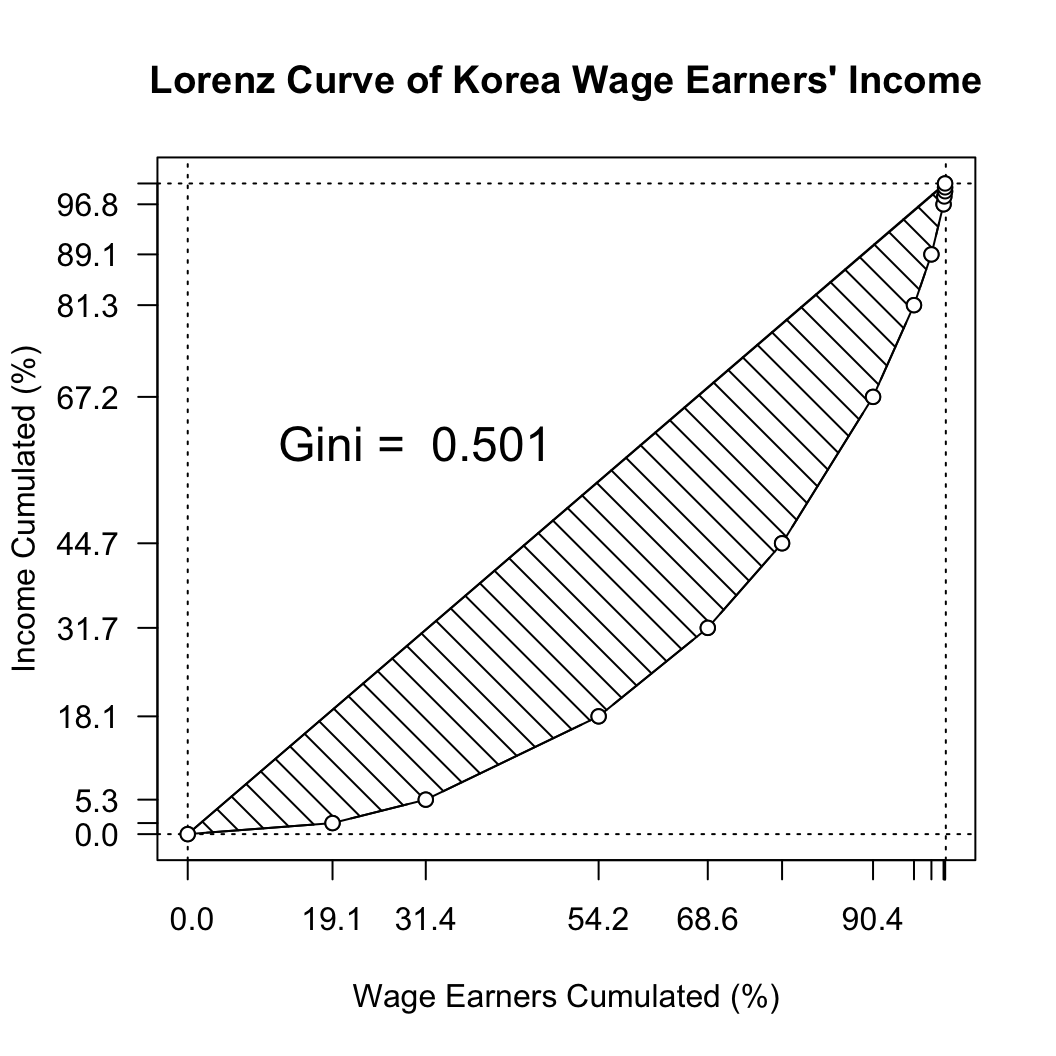
\includegraphics{Gini_OECD_files/figure-latex/unnamed-chunk-19-1.pdf}

\begin{itemize}
\tightlist
\item
  개선도 순서대로 늘어세우려면 그 순서를 \texttt{level}로 갖는
  \texttt{factor}로 만들어야함. \texttt{o\_improvement}가 내림차순으로
  정리되어 있는 순서이기 때문에 \texttt{rev(o\_improvement)}는
  올림차순으로 정리되어 있는 순서임. 따라서,
\end{itemize}

\begin{Shaded}
\begin{Highlighting}[]
\NormalTok{Gini\_b\_a}\SpecialCharTok{$}\NormalTok{Country\_order }\OtherTok{\textless{}{-}} \FunctionTok{factor}\NormalTok{(Gini\_b\_a}\SpecialCharTok{$}\NormalTok{Country, }
                                 \AttributeTok{levels =}\NormalTok{ Gini\_b\_a}\SpecialCharTok{$}\NormalTok{Country[}\FunctionTok{rev}\NormalTok{(o\_improvement)])}
\CommentTok{\# Gini\_b\_a\_order\_melt \textless{}{-} melt(Gini\_b\_a, }
\CommentTok{\#                             id.vars = "Country\_order", }
\CommentTok{\#                             measure.vars = c("Before", "After"), }
\CommentTok{\#                             variable.name = "Tax", }
\CommentTok{\#                             value.name = "Gini\_Coef")}
\CommentTok{\# str(Gini\_b\_a\_order\_melt)}
\NormalTok{Country\_order }\OtherTok{\textless{}{-}} \FunctionTok{rep}\NormalTok{(Gini\_b\_a[, }\StringTok{"Country\_order"}\NormalTok{], }\AttributeTok{length.out =}\NormalTok{ N)}
\NormalTok{Tax }\OtherTok{\textless{}{-}} \FunctionTok{gl}\NormalTok{(}\DecValTok{2}\NormalTok{, }\FunctionTok{length}\NormalTok{(Gini\_b\_a[, }\StringTok{"Country\_order"}\NormalTok{]), N, }
          \AttributeTok{labels =} \FunctionTok{c}\NormalTok{(}\StringTok{"Before"}\NormalTok{, }\StringTok{"After"}\NormalTok{)) }
\NormalTok{Gini\_b\_a\_order\_tbl }\OtherTok{\textless{}{-}} \FunctionTok{data.frame}\NormalTok{(Country\_order, Gini\_Coef, Tax)}
\end{Highlighting}
\end{Shaded}

\begin{itemize}
\tightlist
\item
  \texttt{Gini\_b\_a\_order\_tbl}의 \texttt{Country\_order}가 개선도
  올림차순으로 정리되어 있는 \texttt{factor}이기 때문에 그대로 활용하면
  됨.
\end{itemize}

\begin{Shaded}
\begin{Highlighting}[]
\FunctionTok{ggplot}\NormalTok{(}\AttributeTok{data =}\NormalTok{ Gini\_b\_a\_order\_tbl, }
       \AttributeTok{mapping =} \FunctionTok{aes}\NormalTok{(}\AttributeTok{x =}\NormalTok{ Country\_order, }
                     \AttributeTok{y =}\NormalTok{ Gini\_Coef, }
                     \AttributeTok{fill =}\NormalTok{ Tax)) }\SpecialCharTok{+} 
  \FunctionTok{geom\_bar}\NormalTok{(}\AttributeTok{stat =} \StringTok{"identity"}\NormalTok{, }
           \AttributeTok{position =} \StringTok{"identity"}\NormalTok{, }
           \AttributeTok{na.rm =} \ConstantTok{TRUE}\NormalTok{) }\SpecialCharTok{+}
  \FunctionTok{geom\_hline}\NormalTok{(}\AttributeTok{yintercept =} \FloatTok{0.4}\NormalTok{, }
             \AttributeTok{color =} \StringTok{"red"}\NormalTok{, }
             \AttributeTok{linetype =} \DecValTok{3}\NormalTok{, }
             \AttributeTok{size =} \DecValTok{1}\NormalTok{) }\SpecialCharTok{+}
  \FunctionTok{scale\_fill\_manual}\NormalTok{(}\AttributeTok{values =} \FunctionTok{c}\NormalTok{(}\StringTok{"darkgrey"}\NormalTok{, }\StringTok{"blue"}\NormalTok{)) }\SpecialCharTok{+}
\CommentTok{\#   scale\_fill\_brewer(type = "qual", palette = "Set1", direction = {-}1) +}
  \FunctionTok{labs}\NormalTok{(}\AttributeTok{title =} \StringTok{"OECD Gini Coefficient"}\NormalTok{, }
       \AttributeTok{subtitle =} \StringTok{"Before and After Tax"}\NormalTok{, }
       \AttributeTok{y =} \StringTok{"Gini Coefficient"}\NormalTok{) }\SpecialCharTok{+}
  \FunctionTok{theme}\NormalTok{(}\AttributeTok{plot.title =} \FunctionTok{element\_text}\NormalTok{(}\AttributeTok{size =} \DecValTok{15}\NormalTok{, }\AttributeTok{hjust =} \FloatTok{0.5}\NormalTok{),}
        \AttributeTok{plot.subtitle =} \FunctionTok{element\_text}\NormalTok{(}\AttributeTok{size =} \DecValTok{10}\NormalTok{, }\AttributeTok{hjust =} \FloatTok{0.5}\NormalTok{)) }\SpecialCharTok{+}
\FunctionTok{coord\_flip}\NormalTok{()}
\end{Highlighting}
\end{Shaded}

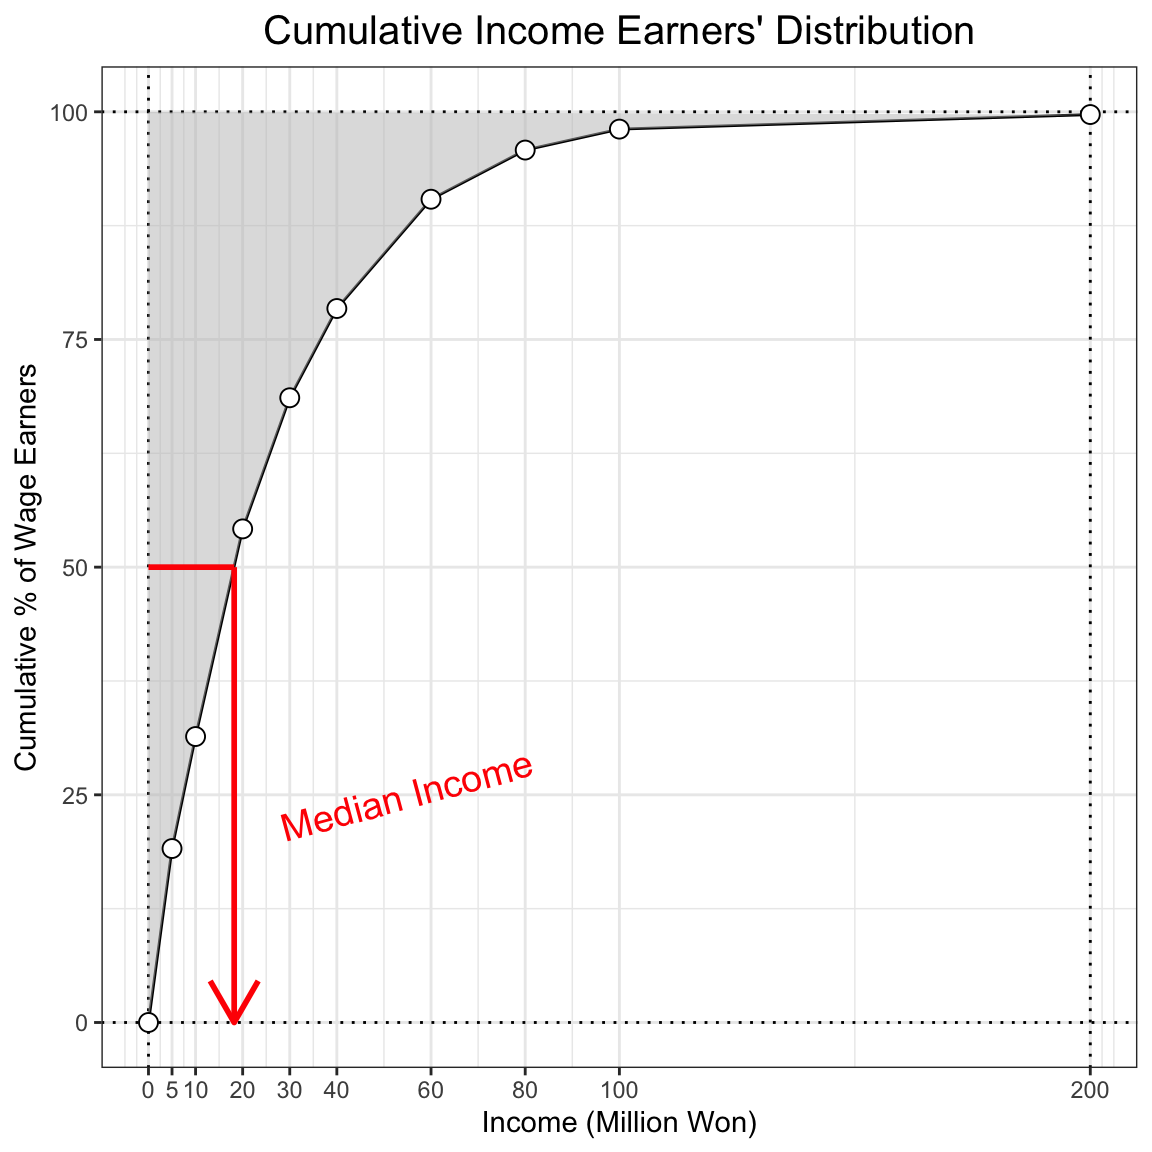
\includegraphics{Gini_OECD_files/figure-latex/unnamed-chunk-21-1.pdf}

\begin{itemize}
\tightlist
\item
  한글 제목 등의 세부 작업은 차후에
\end{itemize}

\hypertarget{uxb4b7-uxb9c8uxbb34uxb9ac}{%
\subsection{뒷 마무리}\label{uxb4b7-uxb9c8uxbb34uxb9ac}}

\begin{Shaded}
\begin{Highlighting}[]
\FunctionTok{save.image}\NormalTok{(}\AttributeTok{file =} \StringTok{"Gini\_OECD.RData"}\NormalTok{)}
\end{Highlighting}
\end{Shaded}


\end{document}
